%%
%%% Headers %%% {{{1
\documentclass[12pt,twoside,a4paper,openright]{report}
%\documentclass[draft,12pt,twoside,a4paper,openright]{report}
%\newcommand{\Hum}{}
\newcommand{\Hum}{\Red{hum hum}\ }
%%
%\newcommand{\Hem}{\Yellow{hem hem}\ }
%\newcommand{\Pics}{\Green{Picture needed}\ }
%% {{{2 Variables definition
\newcommand{\Gael}{Ga\"el Induni}
\newcommand{\thisTitle}{Theoretical study of electronic transport in TCV ELMy H-mode}
\newcommand{\thisTitleBis}{Theoretical study of electronic transport in\\[0.4cm] TCV ELMy H-mode}
%% }}}2
%%
%%% Usepackages %%% {{{2
%%
%% Graphics and figures %% {{{3
\usepackage{graphicx}
\usepackage{wrapfig}
\usepackage{float}
\usepackage{subfig,caption,keyval}
\captionsetup{justification=centering}
%\usepackage{xypic}
%% }}}3
%% Math %% {{{3
\usepackage{amsmath}
\usepackage{amssymb}
%\usepackage{cancel}
%% }}}3
%% Programming %% {{{3
\usepackage{listings}
%\renewcommand{\thelstlisting}{\arabic{section}.\arabic{lstlisting}}
\lstloadlanguages{matlab,Fortran}
\lstdefinestyle{fortran}{
    language        = Fortran,
    numbers         = left,
    numberstyle     = \tiny,
    basicstyle      = \small,
	alsoletter      = {.},
	morekeywords    = {.eq.,.ne.,.gt.,.ge.,.lt.,.le.,.and.,.or.,.true.,.false.},
    keywordstyle    = \bfseries\color{blue},
    identifierstyle = ,
    commentstyle    = \color{red},
    stringstyle     = \color{green},
    showstringspaces= false,
    showspaces      = false,
    frame           = single,
    tabsize         = 2,
    breaklines      = true
}
\lstdefinestyle{matlab}{
    language=Matlab,
    numbers=left,
    numberstyle=\tiny,
    basicstyle=\small,
    keywordstyle=\bfseries,
    identifierstyle=,
    commentstyle=\color{blue},
    stringstyle=,
    showstringspaces=false,
    showspaces=false,
    frame=single,
    breaklines=true
}
%% }}}3
%% Page display %% {{{3
\usepackage{fancyhdr}
\usepackage{hyperref}
%\usepackage[pagebackref]{hyperref}
%\usepackage{multicol}% Remember environement is multicols{n}
%% }}}3
%% Tables %% {{{3
\usepackage{longtable}
\usepackage{multirow}
%\usepackage{colortbl}
%\usepackage{spreadtab}
%\usepackage{numprint}
%% }}}3
%% Bibliography %% {{{3
%\usepackage{doi}
\usepackage[nottoc,chapter]{tocbibind}
\usepackage[nomove,nospace,nobreak]{cite}% superscript
\usepackage[hyperpageref]{backref}
\renewcommand*{\backref}[1]{} 
\renewcommand*{\backrefalt}[4]{
	\ifcase #1
		Not cited.
	\or
		Cited on page~#2.
	\else
		Cited on pages~#2.
	\fi
}
%\renewcommand*{\backrefalt}[4]{
	%\ifcase #1
		%Not cited.
	%\or
		%\ifcase #3
		%\or
			%Cited on page~#2.
		%\else
			%#3 citations on page~#2.
		%\fi
	%\else
		%#3 citations on pages~#2.
	%\fi
%}
%\usepackage{citeref}
%% }}}3
%% Miscellaneous %% {{{3
%\usepackage{alltt}
\usepackage{color}
%\usepackage{everysel,ragged2e}
%\usepackage{gensymb}
%\usepackage{marvosym}
\usepackage{nicefrac}
%% }}}3
\usepackage[english]{babel}
%% hypersetup {{{3
\hypersetup{
	colorlinks        = false,
	bookmarks         = true,
	bookmarksnumbered = true,
	linkcolor         = red,
	urlcolor          = blue,
	filecolor         = blue,
	citecolor         = green,
	hyperfigures      = true,
	breaklinks        = true,
	ps2pdf,
	pdfinfo           = {
		title           = {\thisTitle},
		author          = {\Gael},
		subject         = {\thisTitle},
		displaydoctitle = true,
		keywords        = {plasma} {transport} {diffusion} {H-mode} {pedestal} {ELM} {MHD} {ASTRA} {simulation}
	}
}
\newcommand{\mail}[1]{\href{mailto:#1}{#1}}
\newcommand{\ftplink}[1]{\href{ftp://#1}{#1}}
\newcommand{\myurl}[1]{\href{#1}{#1}}
%% }}}3
%% For my AllFigs environment {{{3
\usepackage{substr}
\usepackage{ifthen}
\usepackage{fixltx2e}
\MakeRobust{\BehindSubString}
\MakeRobust{\BeforeSubString}
\usepackage{tokenizer}
%% }}}3
%%% End of usepackages %%% }}}2
%%
%%% Document size %%% {{{2
%%
\setlength{\topmargin}{-1.25cm}
\setlength{\textheight}{24.5cm}
\setlength{\hoffset}{-1cm}
\setlength{\textwidth}{17cm}
\setlength{\evensidemargin}{0.38cm}
%%
%%% End of document size %%% }}}2
%%
%%% Fancy %%% {{{2
%%
\pagestyle{fancy}
\fancyhead[LO,RE]{\Gael}
\chead{}
\fancyhead[RO]{\thisTitle}
\fancyhead[LE]{\nouppercase{\leftmark}}
\fancyfoot[LO,RE]{\footnotesize 
\includegraphics[width=1cm]{../pics/EPFLno.eps} 
\includegraphics[width=5mm]{../pics/CRPP_Logo.eps} CRPP-EPFL}
\cfoot{}
\fancyfoot[RO,LE]{\thepage}
%%
%%% End of fancy %%% }}}2
%%
%%% Renewing some commands %%% {{{2
%%
%% Ruler for footer and header
\renewcommand{\headrulewidth}{0.4pt}
\renewcommand{\footrulewidth}{0.4pt}
%% Variable that defines where to put floats
\renewcommand{\topfraction}{0.85}
\renewcommand{\textfraction}{0.1}
\renewcommand{\floatpagefraction}{0.75}% < topfraction
%%
%%% End of renrewing commands %%% }}}2
%%
%%% New commands %%% {{{2
%%
\newcommand{\Figref}[1]{Fig.~\ref{fig:#1}}
\newcommand{\figref}[1]{fig.~\ref{fig:#1}}
\newcommand{\Figsref}[1]{Figs.~\ref{fig:#1}}
\newcommand{\figsref}[1]{figs.~\ref{fig:#1}}
\newcommand{\figres}[1]{fig.~\ref{fig:results:#1}}
\newcommand{\tabref}[1]{Tab.~\ref{tab:#1}}
\newcommand{\paref}[1]{\S\ref{sec:#1}}
\renewcommand{\vec}[1]{\mathbf{#1}}
\newcommand{\mat}[1]{\underline{\underline{#1}} }
\newcommand{\Rey}{\mathcal{R}e}
\newcommand{\alali}{\\ \hline}
\newcommand{\dd}{\textrm{d}}
\newcommand{\intdd}[1]{\int\dd #1\ }
\newcommand{\intddlim}[2]{\int\limits_{#2}\dd #1\ }
\newcommand{\intddlims}[3]{\int\limits_{#2}^{#3}\dd #1\ }
\newcommand{\bra}[1]{\left\langle #1\ \right|}
\newcommand{\ket}[1]{\left|\ #1 \right\rangle}
\newcommand{\braket}[2]{\left\langle #1\ |\ #2 \right>}
\newcommand{\ketbra}[2]{\left|\ #1 \rangle\langle #2\ \right|}
\newcommand{\avg}[1]{\left\langle #1 \right\rangle}
\newcommand{\grad}{\nabla}
\renewcommand{\div}{\grad \cdot}
\newcommand{\curl}{\grad \times}
\newcommand{\crossp}[2]{#1 \times #2}
\newcommand{\crosspv}[2]{\vec{#1} \times \vec{#2}}
\newcommand{\dsd}[2]{\dfrac{\partial #1}{\partial #2}}
\newcommand{\dsds}[2]{\frac{\partial #1}{\partial #2}}
\newcommand{\ddsd}[2]{\dfrac{\dd #1}{\dd #2}}
\newcommand{\ddsds}[2]{\frac{\dd #1}{\dd #2}}
\newcommand{\dsdt}[1]{\dsd{#1}{t}}
\newcommand{\dsdts}[1]{\dsds{#1}{t}}
\newcommand{\ddsdt}[1]{\ddsd{#1}{t}}
\newcommand{\ddsdts}[1]{\ddsds{#1}{t}}
\newcommand{\DsDtexpl}[2]{\dsdt{#1} + ( #2 \cdot \grad ) #1}
\newcommand{\DsDt}[1]{\dfrac{D #1}{D t}}
\renewcommand{\epsilon}{\varepsilon}
\renewcommand{\approx}{\simeq}
\renewcommand{\roman}{\Roman}
\makeatletter
\newcommand{\Rom}[1]{\expandafter\@slowromancap\romannumeral #1@}
\makeatother
\newcommand{\Yellow}[1]{\colorbox{yellow}{#1}}
\newcommand{\Green}[1]{\colorbox{green}{#1}}
\newcommand{\Red}[1]{\colorbox{red}{#1}}
\newcommand{\Blue}[1]{\colorbox{blue}{#1}}
\newcommand{\Par}{/\!/}
%%
%% New commands for figs environments {{{3
\newcommand{\resultsplot}[4]{\subfloat[]{\includegraphics[width=7cm]{../matlab/pics/40080_0.8_#4_#3_results_#1.eps}\label{fig:results:ELMs:#1:#2:#4}} }
\newcommand{\resultsplotO}[1]{\subfloat[]{\includegraphics[width=7cm]{../matlab/pics/40080_0.8_#1_results_cycle.eps}\label{fig:results:ELMs:cycle:#1}} }
\newcommand{\rhosOKplot}[2]{\subfloat[]{\includegraphics[width=7cm]{../matlab/pics/40080_0.8_#2_rhosOK_#1.eps}\label{fig:results:ELMs:rhosOK:#1:#2}} }
%% }}}3
%% AllFigs {{{3
\newcounter{maxFigs}
\newcounter{coFigs}
\newcounter{KeepSubFig}
\newcommand{\Argv}{}
\newcommand{\tmpArgv}{}
\newcommand{\tmpArgvBis}{}
\newcommand{\thisArg}{}
\newcommand{\ParsChar}{,}
\newcommand{\PutLabel}{}
\newcommand{\InLabel}{}
\newcommand{\Plural}{s}
\newcommand{\Grammar}{}
\newcommand{\GrammarVerb}{are}
\newcommand{\ResultsComment}{ The left figure\Plural\ show\Grammar\ the traces at the top of the density pedestal while the right one\Plural\ \GrammarVerb\ at the maximum of the pressure gradient.}
\newcommand{\TheCap}{}
%% 1: case, 2: fig position, 3: , 4: quantities to display, 5: continued, 6: candidate (resultplot/resultplotO/rhosOKplot), 7: caption
\newenvironment{AllFigs}[7]{
	\renewcommand{\Argv}{#4}
	\renewcommand{\thisArg}{}
	\IfSubStringInString{\ParsChar}{\Argv}{%
		\SubStringsToCounter{maxFigs}{\ParsChar}{\Argv}%
		\addtocounter{maxFigs}{2}%
	}{%
		\setcounter{maxFigs}{2}%
	}
	\setcounter{coFigs}{1}
	\ifthenelse{\equal{#5}{y}}{%
		\setcounter{subfigure}{\theKeepSubFig}%
	}{}
	\begin{figure}[#2]
	\begin{center}
	\ifthenelse{\equal{#5}{y}}{\ContinuedFloat}{}
	\whiledo{\thecoFigs < \themaxFigs}{
		\IfSubStringInString{\ParsChar}{\Argv}{%
			\let\tmpArgv\Argv
			\GetTokens{thisArg}{Argv}{\tmpArgv}
		}{%
			\renewcommand{\thisArg}{\Argv}%
		}
		\ifthenelse{\equal{#6}{resultsplotO}}{%
			\resultsplotO{\thisArg}%
			\ifthenelse{\equal{\Argv}{\thisArg}}{}{%
				\ifthenelse{ \isodd{\thecoFigs}}{\hspace{2mm}}{\linebreak}%
			}
		}{%
			\ifthenelse{\equal{#6}{resultsplot}}{%
				\ifthenelse{\equal{\thisArg}{ibsped}}{%
					\resultsplot{#1}{ped}{0.860}{\thisArg}
				}{%
					\resultsplot{#1}{core}{0.754}{\thisArg}\hspace{2mm}
					\resultsplot{#1}{ped}{0.860}{\thisArg}
				}
				\ifthenelse{\equal{\thisArg}{\Argv}}{}{\linebreak}%
			}{%
				\rhosOKplot{#1}{\thisArg}
				\ifthenelse{\equal{\Argv}{\thisArg}}{}{%
					\ifthenelse{ \isodd{\thecoFigs}}{\hspace{2mm}}{\linebreak}%
				}
			}%
		}
		\stepcounter{coFigs}
	}
	\vspace{-6mm}
	\end{center}
	% label
	\ifthenelse{\equal{#5}{y}}{
		\renewcommand{\InLabel}{none}%
	}{%
		\ifthenelse{\equal{#6}{resultsplotO}}{%
			% cycle
			\renewcommand{\InLabel}{cycle}
		}{%
			\ifthenelse{\equal{#6}{resultsplot}}{%
				% results
				\renewcommand{\InLabel}{#1}
			}{%
				% rhosOK
				\renewcommand{\InLabel}{rhosOK:#1}
			}%
		}
	}
	\ifthenelse{\equal{#5}{a}}{%
		\let\tmpInLab\InLabel%
		\renewcommand{\InLabel}{\tmpInLab:app}%
	}{}
	\ifthenelse{\equal{\InLabel}{none}}{%
		\renewcommand{\PutLabel}{}
	}{%
		\renewcommand{\PutLabel}{\label{fig:results:ELMs:\InLabel}}
	}
	% Caption
	\renewcommand{\TheCap}{#7}
	\ifthenelse{\equal{#6}{resultsplot}}{%
		\ifcase \themaxFigs
		\or \or
			\renewcommand{\Plural}{}
			\renewcommand{\Grammar}{s}
			\renewcommand{\GrammarVerb}{is}
		\else
			\renewcommand{\Plural}{s}
			\renewcommand{\Grammar}{}
			\renewcommand{\GrammarVerb}{are}
		\fi
		\renewcommand{\TheCap}{#7\ResultsComment}
	}{}
	\caption{\footnotesize \TheCap\PutLabel}
	%\caption{\footnotesize #7 (Colors in the electronic version.)\PutLabel}
	\vspace{-5mm}
	\end{figure}
}{
	\ifthenelse{\arabic{subfigure} > 0}{%
		\setcounter{KeepSubFig}{\arabic{subfigure}}%
		\setcounter{subfigure}{0}%
	}{}
}
%% }}}3
%% New commands for references {{{3
\newcommand{\AllFigsRef}[1]{\ref{fig:results:ELMs:#1}}
\newcommand{\AllFigsRefO}[1]{\ref{fig:results:ELMs:cycle#1}}
\newcommand{\AllProfsRef}[1]{\ref{fig:results:ELMs:rhosOK:#1}}
\newcommand{\AllFigsSub}[1]{\subref*{fig:results:ELMs:#1}}
\newcommand{\AllFigsSubO}[1]{\subref*{fig:results:ELMs:cycle:#1}}
\newcommand{\AllProfsSub}[1]{\subref*{fig:results:ELMs:rhosOK:#1}}
%% }}}3
%%
%%% End of new commands %%% }}}2
\newcommand{\tauELM}{100}
\newcommand{\deltaELM}{20}
\newcommand{\fELM}{50}
\newcommand{\Shot}{40080}
\newcommand{\tZero}{0.8}
\newcommand{\Zeff}{2.9}
\newcommand{\deltaST}{6}

%%
\setcounter{tocdepth}{1}
\numberwithin{equation}{chapter}
%% }}}1
%%
\begin{document}
%%
%%% Title page %%% {{{1
%%
\pagestyle{empty}
\renewcommand{\thepage}{\alph{page}}
\begin{titlepage}
%\setcounter{page}{-1}
\begin{center}
{\Huge \thisTitleBis}\\[1.8cm]
{\Large \Gael}\\[0.7cm]
{\mail{gael.induni@epfl.ch}}\\[1.5cm]
%%{\large CRPP, EPFL}\\[6cm]
\begin{minipage}[c]{0.52\textwidth}
\begin{flushright}

\includegraphics[width=3cm]{../pics/EPFL.eps}
\end{flushright}
\end{minipage}
\hspace{1cm}
\begin{minipage}[c]{0.4\textwidth}
\begin{flushleft}

\includegraphics[width=1.5cm]{../pics/CRPP_Logo.eps}
\end{flushleft}
\end{minipage}
\end{center}
\vspace{2cm}
\begin{center}
Master's thesis
\end{center}
\vspace{3cm}
\begin{flushright}
\large Supervisor:\\
Olivier Sauter\\
{\small \mail{olivier.sauter@epfl.ch}}
\end{flushright}
\vfill
\begin{center}
\today
\end{center}
\end{titlepage}
\cleardoublepage
%% }}}1
%% Abstract {{{1
\pagestyle{fancy}
\renewcommand{\thepage}{\Roman{page}}
\setcounter{page}{1}
\setlength{\parskip}{0.5ex}
\chapter*{Abstract}\label{sec:abs}\thispagestyle{fancy}
\addcontentsline{toc}{chapter}{Abstract}
%%
High-confinement mode (H-mode) is a promising reference scenario for ITER. But we are still facing major issues because of instabilities. They expel periodically some of the energy, which can damage the device. These instabilities are called the edge localized modes (ELM) and are not yet fully theoretically understood.

The present work is a study on the profiles evolution in between ELMs and on the ELM effects. This may help to have a better understanding of the conditions before the ELM. We use the simulations as theoretical tool.

For the purpose of the simulations, we build an H-mode $\chi_e$ profile according to a standard L-mode one that we truncate at the edge to create a transport barrier. This gives a good agreement with the experimental data.

Several scaling laws were successfully used. The first one is the energy confinement time scaling which was used for the thermal diffusivity to scale the temperature profile. A scaling between the core and pedestal energies was found recently. It was used to compute the pedestal $\chi_e$ to scale the temperature pedestal, which was successful. Finally, we used a scaling for transport barriers which links the density gradient length to that of the temperature to compute the density in the pedestal. It was already found to be good in TCV electron internal transport barriers and in ASDEX Upgrade H-mode pedestals.

Looking at the MHD stability parameters, it was found that for our reference case, ELMs are not likely to be triggered by the time evolution of the pressure gradient and the current density profiles in our model, as these are only varying significantly during the first millisecond after the crash, and are almost constant during the long remaining time until the next crash.

Studying different cases, we investigate the behavior of the plasma when replacing the edge heating by central one to observe the influence of the heating profile, but no significant difference was found, neither in the MHD stability parameters.

Further we change the particle diffusion coefficient to compare the dynamic behavior of the density. Slowing down the density dynamic behavior also slows down the pressure one, this can be seen on the MHD stability parameters. We also vary the ELM period to compare to the change due to the variation of the particle diffusivity. It was found that there may be a sort of relation between the particle diffusivity and the ELM period at least for the density, since both cases change the density recovery time with respect to the ELM period.

A last case considered is doubling the radial ELM interaction range. This is done in order to observe the difference to the reference simulation that takes the density top of pedestal as ELM range, and to compare the spatial range influenced by the MHD activity and the one by the transport improvement. It was found that the MHD stability parameters in the pedestal exhibit a different behavior with the pressure gradient starting to increase very fast.

\cleardoublepage
%% }}}1
%% TOC {{{1
\setlength{\parskip}{0ex}
\tableofcontents
\thispagestyle{fancy}
\setlength{\parskip}{0.5ex}
\cleardoublepage
\renewcommand{\thepage}{\arabic{page}}
\setcounter{page}{1}
%% }}}1
%%
\chapter{Introduction}\thispagestyle{fancy}
%%
Fusion may be our future source of energy. For now, we are not able to achieve it in an economically viable way because we do not understand fully what happens in our tokamaks. A long time ago, Lawson was also working on fusion research. He predicted that we will face some problems he did not know at that moment. This was very smart of him. He also predicted from where those problems will arise: ``Conduction loss is difficult to treat in a general way, since it depends on the geometry of the system, its density and temperature distribution, and also the wall material.'' \cite{lawson}\ Actually the wall material has not much to do with the losses, or indirectly. Nowadays we are facing problems coming from within the plasma, instabilities and turbulence.

As the research went further on fusion, we discovered some limitations to our reactors. Looking for a way to overcome them, it was once discovered in ASDEX a regime where the confinement is improved by about a factor two \cite{iterNews}. This was done twenty-nine years ago. This operation mode was not predicted, but it appeared for a sufficient input power. It is called the H-mode, standing for \emph{High-confinement mode}, in opposition to the \emph{Low-confinement mode} (L-mode). Since then this promising operational mode has been studied extensively.

We then discovered that one of the features of H-mode is the instabilities called edge localized modes (ELMs). ELMs expel periodically some particles and energy. They are somehow useful, because it helps the plasma expel the impurities, and not to increase too much the density. But there are many types of them, and some expel very large quantities of energy. The expelled particles and energy onto the vessel. This may cause destructive erosion of the plasma-facing components that could make the device not viable.

In order to have a better knowledge of the physics in H-mode, here is studied the electronic transport in the inter-ELM phase. This can be done through theoretical studies to avoid the machine deterioration. We will do a brief overview of the limits responsible for the ELMs, but this work focuses on the profiles evolution in between ELMs and on the ELM effects. This may help us to better understand the conditions before an ELM.

The next step in fusion research is being built in France, the famous International Thermonuclear Experiment Reactor (ITER). Its operational scenario is an ELMy H-mode. It is therefore of prime importance to have a better knowledge of the transport in the inter-ELM phase.

This work will first recall some theory basis that are needed. We will do an overview of the magnetohydrodynamics theory and instabilities. Then we will speak about the plasma confinement, more specifically of the transport phenomena, leading to the H-mode description. This study being theoretical, we then explain the tool used in this work and how the implementation has been achieved. Finally, different cases were studied and comparisons between these results are presented. We will study the inter-ELM profiles, time traces and the MHD stability diagrams.

%%
\chapter{Magnetohydrodynamics}\label{sec:MHD}\thispagestyle{fancy}
%% Theory preamble (no section) {{{1
This chapter is not intended to provide a full description of the MagnetoHydroDynamics (MHD) but will only present the part that is necessary to understand this work. For further knowledge, the reader can refer to the books \cite{freidberg,boyd-sanderson,freidberg2,wesson}.

The ideal MHD is based upon conservation laws, the fluid equations and Maxwell's equations \cite{freidberg}. The MHD model is focusing on the characteristic scales of the macroscopic behavior of the plasma. It can be built from the two-fluid model (described in \cite{freidberg}), reducing it to a single-fluid one and completing it with electrodynamics.

The range of validity of ideal MHD is defined upon three parameters: the characteristic length, time and velocity \cite{freidberg}. They are respectively defined by the plasma radius, the ion thermal transit time across the plasma and the characteristic velocity defined by the ratio of the two previous parameters. Indeed, in ideal MHD it mainly depends on the plasma radius $a$ and on the ion sound speed $v_{T_i}$ because we define the characteristic time as $\tau = a / v_{T_i}$ and the velocity $u = a / \tau = v_{T_i}$.

Taking in consideration the electromagnetic quantities, it yields three conditions \cite{freidberg}:
\begin{description}
	\item[Length]    $a \gg r_{L,i} \gg r_{L,e} \sim \lambda_{De}$
	\item[Frequency] $\bar{\nu}_{ei} \ll \dfrac{1}{\tau} = \dfrac{v_{T_i}}{a} \ll \omega_{c,i}$
	\item[Velocity]  $v_{T_i} \ll v_{T_e} \ll c$
\end{description}
where $r_L$ is the Larmor radius, $\lambda_{De}$ the Debye length, $\bar{\nu}_{ei}$ the momentum exchange collision frequency and $\omega_c$ the cyclotronic frequency. There are some more conditions that fall from these, including that the plasma pressure has to be finite compared to the magnetic pressure, requiring $\beta = p / ( B^2 / 2 \mu_0 ) \sim 1$ \cite{freidberg}.

Introducing the Alfv\'en velocity $v_A^2 = B^2 / ( \mu_o n_i m_i )$, it is approximately equal to $2 v_{T_i}^2 / \beta$, implying that the MHD characteristic timescale $\tau$ is the Alfv\'en time $\tau_A = a / v_A$ \cite{boyd-sanderson}.

We introduce the single-fluid variables as the mass density $\rho$, the fluid (macroscopic) velocity $\vec{u}$ and the pressure \cite{freidberg}. Since a plasma relies on quasi-neutrality meaning $n_e = n_i = n$ and ions having a much larger mass than electrons $m_i \gg m_e$, the mass density is defined as $\rho = m_i n$ and the fluid velocity as $\vec{u} = \vec{v}_i$. The pressure being not so different for the two species, the fluid pressure is simply the sum of both contributions $p = p_i + p_e$.

Electrons and ions flowing in different directions, it creates a current, defined by the current density $\vec{J} = e n (\vec{v}_i - \vec{v}_e)$ which can be used to express the electron velocity as
\begin{align*}
	\vec{v}_e & = \vec{u} - \frac{\vec{J}}{e n}
\end{align*}
Using these variables in the two-fluid model, we can now write the ideal MHD equations \cite{freidberg}:
\begin{align}
	\textrm{Mass conservation}     && \DsDt{\rho} + \rho\ \div \vec{u}               & = 0                                     \label{eq:MHD:mass_cons}\\
	\textrm{Momentum conservation} && \rho\ \DsDt{\vec{u}}                           & = \crossp{\vec{J}}{\vec{B}} - \grad p   \label{eq:MHD:momentum_cons}\\
	\textrm{Ohm's law}             && \vec{E} + \crossp{\vec{u}}{\vec{B}}            & = \eta \vec{J}                          \label{eq:MHD:ohmslaw}\\
	\textrm{Energy}                && \DsDt{} \left( \frac{p}{\rho^{\gamma}} \right) & = 0                                     \label{eq:MHD:energy_cons}\\[2mm]
	\textrm{Maxwell}               && \begin{cases}
											\phantom{a}\\[-12pt]
											\curl \vec{E}\\[2pt]
											\curl \vec{B}\\
											\div  \vec{B}
                                      \end{cases}\!\!\!\!\! &   \begin{array}{l}
																	= - \dsdt{\vec{B}}\\[3pt]
																	= \mu_0 \vec{J}\\[1pt]
																	= 0
																\end{array}\label{eq:MHD:maxwells}
\end{align}
where $\gamma = \nicefrac{5}{3}$, and the convective derivative is expressed as
\begin{align*}
	\DsDt{} = \DsDtexpl{}{\vec{u}}
\end{align*}
Treating the \textbf{ideal} MHD means we consider the plasma as an ideal conductor and therefore set $\eta = 0$, which drops the right-hand side term of \eqref{eq:MHD:ohmslaw}.

What is interesting now is the behavior of such a system to a small perturbation. 
%We now denote without index the quantities from the equilibrium and with index 1 the ones from the perturbation. Moreover we state that the equilibrium is static, meaning $\vec{v} = 0$. We define the perturbation displacement vector as $\xi$ and therefore we have $\vec{v}_1 = \dsdts{\xi}$, and every perturbed quantities can have the temporal dependence removed by a normal mode expansion $Q_1(\vec{r},t) = Q_1(\vec{r}) e^{- i \omega t}$. We can write the linear stability equations \cite{freidberg}:
%\begin{align}
	%\begin{cases}
		%\rho_1    & = - \div \left( \rho \xi \right)\\
		%p_1       & = - \xi \cdot \grad p - \gamma p \div \xi\\
		%\vec{B}_1 & = \curl \left( \crosspv{\xi}{B} \right)\\
		%\vec{J}_1 & = \dfrac{1}{\mu_0} \curl \left( \curl \left( \crosspv{\xi}{B} \right) \right)
	%\end{cases}\label{eq:MHD:lins}
%\end{align}
%This yields a single vector equation
%\begin{align}
	%\rho\ \frac{\partial^2 \xi}{\partial t^2} = \vec{F}(\xi)\label{eq:MHD:eigenval_before}
%\end{align}
%where $\vec{F}$ is a complicated operator deduced from \eqref{eq:MHD:momentum_cons} by linearizing and substituting the perturbed quantities by their meaning found in \eqref{eq:MHD:lins}.
%%
%We assume that we can separate the time and space dependence of the displacement vector as $\xi(\vec{r},t) = \xi(\vec{r}) T(t)$. We choose $T(t) = e^{i \omega t}$ so that $\ddot{T} = - \omega^2 T$ and \cite{boyd-sanderson}
%\begin{align}
	%\xi(\vec{r},t) = \xi(\vec{r}) e^{i \omega t}\label{eq:MHD:xiexp}
%\end{align}
%Equation \eqref{eq:MHD:eigenval_before} then becomes
%\begin{align}
	%- \omega^2 \rho \xi = \vec{F}(\xi)\label{eq:MHD:eigenval}
%\end{align}
%The operator $\vec{F}$ is linear in $\xi$, meaning \eqref{eq:MHD:eigenval} is an eigenvalue problem \cite{boyd-sanderson}. %, where the possible values of $\omega^2$ are determined by the boundary conditions \cite{boyd-sanderson}. 
%For discrete eigenvalues, we can do a normal mode expansion with $\xi_n$ the normal mode associated to the frequency $\omega_n$ \cite{boyd-sanderson}. The general solution becomes
%\begin{align*}
	%\xi(\vec{r},t) = \sum_n \xi_n(\vec{r}) e^{i \omega_n t}
%\end{align*}
%MHD equations have no dissipative term and thus conserve energy \cite{boyd-sanderson}. A stable equilibrium configuration is then reached if the potential energy $W$ is at one of its minima. The energy principle states that the equilibrium is unstable if there exists a displacement vector $\xi$ for which $\delta W < 0$.
%%
%To find this change in potential energy, we compute the change in kinetic energy
%\begin{align*}
	%K(\dot{\xi},\dot{\xi}) & = \frac{\rho}{2} \intdd{V} \dot{\xi} \cdot \dot{\xi} \stackrel{\eqref{eq:MHD:xiexp}}{=} - \frac{\rho \omega^2}{2} \intdd{V} \xi \cdot \xi \stackrel{\eqref{eq:MHD:eigenval}}{=} \frac{1}{2} \intdd{V} \xi \cdot \vec{F}(\xi)
%\end{align*}
%and hence by the energy conservation:
%\begin{align*}
	%\delta W(\xi,\xi) & = - \frac{1}{2} \intdd{V} \xi \cdot \vec{F}(\xi)
%\end{align*}
%Using the operator $K$ with $K(\dot{\xi},\dot{\xi}) = -\omega^2 K(\xi,\xi)$, we can find
%\begin{align*}
	%\omega^2 = \frac{\delta W(\xi,\xi)}{K(\xi,\xi)}
%\end{align*}
%and hence the sign of $\omega^2$ is determined by that of $\delta W$.
%%
%Using the self-adjoint property of $\vec{F}$, we know that its eigenvalues are real \cite{freidberg}. Hence $\omega^2$ can be either positive or negative; a positive $\omega^2$ is linked to the oscillation case, which is stable, but a $\omega^2 < 0$ yields a solution growing exponentially, thus unstable, at a rate $\gamma = \sqrt{-\omega^2}$.
The full development can be found in \cite{freidberg,boyd-sanderson}. It leads to the conclusion that the system is unstable if the change in potential energy $\delta W$ is negative. With appropriate boundary conditions we can decompose it in a plasma, a surface and a vacuum contributions \cite{boyd-sanderson}:
\begin{align*}
	\delta W = \delta W_P + \delta W_S + \delta W_V
\end{align*}
%where these contributions are given by \cite{boyd-sanderson}:
%\begin{align}
	%\delta W_V & =             \int_{V} \dd V\ \frac{\left| \widetilde{\vec{B}}_1 \right|^2}{2 \mu_0}\nonumber\\
	%\delta W_S & = \frac{1}{2} \int_{S} \dd \vec{S}\ \cdot ( \vec{n} \cdot \xi )^2 \nabla \left( p + \frac{B^2}{2 \mu_0} \right)\nonumber\\
	%\delta W_P & = \frac{1}{2} \int_{P} \dd V\ \left( \frac{|\vec{B}_1|^2}{\mu_0} + \gamma\ p |\div \xi|^2 + \vec{j} \cdot ( \xi \times \vec{B}_1 ) + ( \div \xi ) ( \xi \cdot \nabla p ) \right)\label{eq:MHD:deltaWP}
%\end{align}
%where $\widetilde{\vec{B}}_1$ is a perturbation of the vacuum magnetic field, and the integral indices $V, S$ and $P$ correspond to the unperturbed vacuum volume, plasma surface and volume respectively.

Introducing the field curvature $\kappa = ( \vec{b} \cdot \nabla ) \vec{b}$ where $\vec{B} = B \vec{b}$, we can rewrite each vector quantity $\vec{d}$ as a component parallel to the toroidal field $d_{\Par}$ and a perpendicular one $\vec{d}_{\perp}$ which gives the relation $\vec{d} = d_{\Par} \vec{b} + \vec{d}_{\perp}$. Hence we may write the plasma contribution as \cite{boyd-sanderson}
\begin{align}\nonumber
	\delta W_P = \frac{1}{2} \int_{P} \dd V\ \bigg( & \frac{B_{1,\perp}^2}{\mu_0} + \frac{B^2}{\mu_0} \left( \div \xi_{\perp} + 2 \xi_{\perp} \cdot \kappa \right)^2 + \gamma\ p (\div \xi)^2\\
												    & - 2 ( \xi_{\perp} \cdot \nabla p ) ( \kappa \cdot \xi_{\perp} ) - j_{\Par} ( \xi_{\perp} \times \vec{b} ) \cdot \vec{B}_{1,\perp} \bigg)
	\label{eq:MHD:deltaWP2}
\end{align}
where the quantities without index are from the equilibrium whereas those with index 1 are the perturbed ones, $\vec{J} \simeq j_{\Par} \vec{b}$ and $\xi$ is the perturbation displacement defined by
\begin{align}
	\xi(\vec{r},t) & = \xi(\vec{r}) e^{i \omega t}           \label{eq:MHD:xiexp}% REMOVE THIS IF UNCOMMENTING ABOVE
\end{align}

We usually have no currents flowing on the plasma surface and thus the surface term vanishes. The $\delta W_V$ represents the perturbed magnetic vacuum energy. An ideal conducting wall near the plasma has a stabilizing effect, as it is the vacuum region that destabilizes.

The plasma perturbed energy contains many terms. The two first ones are linked to the bending of the magnetic field lines. They are always positive and therefore stabilizing. The third term represents the energy needed by the plasma to be compressed, it is also a stabilizing term.

The last two terms are proportional to $\vec{j}$ and $\nabla p$ and thus can be either positive or negative. If negative, instabilities will arise. There are lots of them and they can be characterized in different ways. Those caused by the pressure gradient term are often called \emph{pressure-driven} modes, while instabilities caused by the parallel currents are called \emph{current-driven} modes \cite{boyd-sanderson,freidberg}. This denomination means that those instabilities can arise even though the other destabilizing term does not act. For instance, current-driven modes can exist in the low $\beta$ limit where all the pressure-modes are stabilized. Nevertheless, we usually have both pressure gradient and current density contributions together.
%% }}}1
%%%%%%%%%% SECTION %%%%%%%%%% {{{1 MHD stability parameters
\section{MHD stability parameters}\label{sec:MHD:qqs}
%%
With coordinates $(R,\phi,z)$ and using the relation $\vec{B} = \curl \vec{A}$, we can define the \emph{poloidal flux} $\psi = R A_{\phi}$, yielding $(\vec{B} \cdot \nabla) \psi = 0$ \cite{boyd-sanderson}. This means that the poloidal flux is constant along the magnetic surfaces and therefore $\psi$ can be used as a coordinate. We can show after some algebra that surfaces of constant $\psi$ are also surfaces of constant current and of constant pressure \cite{boyd-sanderson}.

We define the ratio of change of the magnetic helicity in toroidal angle to that of the poloidal angle as \cite{boyd-sanderson}
\begin{align}
	q & = \frac{1}{2 \pi} \oint\limits_{poloidal \atop circuit} \dd l\ \frac{B_t}{R B_p}   \label{eq:MHD:stab:q}
\end{align}
where $B_t$ and $B_p$ are respectively the toroidal and the poloidal magnetic field. The latter is created by the plasma current. This ratio can hence be seen as
\begin{align*}
	q & = \dfrac{\Delta \phi}{2 \pi}
\end{align*}
where $\Delta \phi$ is the change in toroidal angle for a change of $2 \pi$ in poloidal angle along a magnetic surface. If $q$ is rational, we can write $q = m / n$ where $m$ and $n$ are integers, meaning that the magnetic field lines join themselves after $m$ toroidal revolutions and $n$ poloidal ones. Hence the field lines are joining themselves after a finite number of revolutions. If we recall of \eqref{eq:MHD:xiexp}, we can also see $m$ and $n$ as the poloidal and toroidal mode number respectively \cite{gimblett2006}:
\begin{align*}
	\xi(\vec{r}) & = \sum_{m,n} \hat{\xi}_{m,n}(r) e^{ i ( n \phi + m \theta ) }
\end{align*}

At a given equilibrium, $q$ has a fixed profile, but the mode numbers can be numerous. This means that, at a given location, we have a variety of mode numbers for a single value of $q$, linking the toroidal mode number to the poloidal one by the relation $ q = m / n$.

The instabilities following the field lines, we understand that the joining of the latter will help the instabilities to grow up. Thus rational values of $q$ are dangerous for the plasma stability. This ratio $q$ is an important parameter of MHD stability and is called the \emph{safety factor}.

The shear of a vector $\vec{F}$ is defined as $\nabla \vec{F}$. The magnetic shear $s$ is the shear of the safety factor. As the latter is radial and we are only interested in the radial direction, we define the magnetic shear $s = s(\rho)$ as
\begin{align*}
	s = \frac{\rho}{q} \ddsd{q}{\rho}
\end{align*}
$\rho$ being the radial coordinate. The higher the magnetic shear, the lower the radial transport. Thus high values of the shear have a stabilizing effect on the plasma.
%% }}}1
%%%%%%%%%% SECTION %%%%%%%%%% {{{1 Instabilities
\section{Instabilities}\label{sec:MHD:instab}
%%
Instabilities are numerous in the MHD theory. We do not intend to describe all of them in this work, but H-mode plasmas deal with some that may be recalled here.

Looking at \eqref{eq:MHD:deltaWP2}, we have discussed the last two terms about their capability of destabilization. The first one concerns the pressure. If we have a pressure gradient $\grad p$ and a magnetic field curvature $\kappa$ in the same direction, we understand that this term will be destabilizing. Tokamaks have a curvature aimed at their center, and the pressure gradient is generally directed towards the center of the plasma. On the inner part of the tore, $\nabla p$ and $\kappa$ are aiming at different directions. But looking at the outer part, both $\nabla p$ and $\kappa$ are directed towards the center of the plasma. This yields that the destabilization-drive is mainly on the outer part and the perturbation amplitude tends to maximize them.

Such perturbations are called the \emph{ballooning modes} in the $n \rightarrow \infty$ limit. The ballooning stability parameter is defined by the normalized pressure gradient
\begin{align*}
	\alpha = - R_0 q^2 \ddsd{\beta}{r}
\end{align*}
where $R_0$ is the major radius of the tokamak and $r$ the metric radius of the plasma.

%These are external modes, meaning the main destabilization comes from the vacuum between the plasma and the wall. This implies that the vacuum and surface energy differences are non-zero and must be evaluated. Suppressing this vacuum by nearing the wall would stabilize these modes.
%%
For finite $n$, we encounter some other modes called \emph{external kink}. These modes are more difficult to understand, but the literature provides documentation, e.g. references \cite{wesson1978,lortz1975}. Considering the second-order potential energy, the destabilizing term is the radial gradient of toroidal current density $\dd j_t / \dd r$ \cite{wesson1978}.

The origin of this term comes from the properties of the kink modes. They are incompressible and therefore need a torque to kink. The latter is provided by the $\crosspv{j}{B}$ force. The torque being the curl of the force, the gradient of the current density appears in the torque, hence driving the instability. However, this term is also present in the magnetic shear, which has a stabilizing effect \cite{wesson1978}. We must ask ourselves what are the conditions for this destabilizing force to become an instability.

Considering first no vacuum between the plasma and the wall, we find after some algebra that the destabilizing term in the potential energy is $j_{t,a} / \avg{j_t}$, the index $a$ referring to the edge value and $\avg{\cdot}$ being the volume average. Thus the stability criterion in this limit is given by $j_{t,a} \le 0$. This limit case is the same when the wall is further for $m \rightarrow \infty$ modes. Looking at finite high $m$ modes, further analysis yields an additional stability criterion as
\begin{align*}
	\left. \dsd{j_t}{r} \right|_a = 0
\end{align*}

The edge current density plays an important role for these modes \cite{connor1998}. In particular the bootstrap current (see \paref{confinement:transport}) has a destabilizing effect on the external kink \cite{gimblett2006}. It is thus understandable that H-mode will often have to face them because of the pressure pedestal which implies the arising of the edge pressure gradient and thus a finite edge current density.

In the H-mode regime, the most common instabilities are non-negligible. They are called edge localized modes (ELM). They are characterized by the emission of $H_{\alpha}$ radiation \cite{wesson}. They are not yet fully understood but are believed to be due to the combination of the ballooning modes and the external kink \cite{loennroth2004}.

There are many types of these ELMs but we will only discuss about type-I and type-III ELMs. The main difference between these two types is the occurrence of the ELMs according to the input power. Type-I ELMs increase their frequency with respect to the input power whereas type-III ELMs decrease theirs. Type-I ELMs are very large ELMs and are very dangerous for the plasma facing-components due to the large energy loss ($\Delta W / W \simeq 8 - 25 \%$ \cite{andreas2010}) that go directly onto the divertor plates \cite{wesson}. The latter type being the most dangerous for the machine, this study is focused on them.

ELMs do not have a specific stability parameter but are studied using the stability parameters of both ballooning modes and external kink, respectively $\alpha$ and $j_{t,a}$. The proper way to observe the evolution of the plasma among the ELMs is using a diagram of $j_{t,a}$ as function of $\alpha$, where we have a stability region for the plasma.

Another instability often present in tokamak plasmas is the sawtooth instability. It is an internal instability and is supposed to be due to the internal kink. This mode is described by $n = 1, m = 1$. This means the $q = 1$ surface plays an important role since the instability occurs inside it. We denote the radius of this surface by $r_1$. $q = 1$ is the surface where the magnetic toroidal angle is equal to the poloidal one, joining the field lines after a single revolution of the machine only. Therefore the small instabilities are allowed to grow very much because they follow the same magnetic field line for many revolutions.
%% }}}1

\chapter{Plasma confinement}\label{sec:confinement}\thispagestyle{fancy}
%%
%%%%%%%%%% SECTION %%%%%%%%%% {{{1 Transport
\section{Transport}\label{sec:confinement:transport}
%%
%Lawson stated a criterion for any device to achieve fusion \cite{wesson}:
%\begin{align*}
	%n \tau_E T & > 5 \cdot 10^{-21} m^{-3} s\ keV
%\end{align*}
%%
The transport of energy and particle are governed by the conservation laws \cite{heatDiff,fable2006}
\begin{align}
	\dsdt{W_j} + \frac{1}{V'} \dsd{}{\rho} \left( V' q_j \right) & = S_j                                      & j = i,e \label{eq:confinement:transport:heat:heatDiff}\\
	\frac{1}{V'} \dsdt{} \left( V' n_e \right) + \frac{1}{V'} \dsd{}{\rho} \left( V' \Gamma_n \right) & = S_n           \label{eq:confinement:transport:particle:particleDiff}
\end{align}
where $W_j = \frac{3}{2} \intdd{V} n_j T_j$ with $j = e,i$, $S_j$ and $S_n$ denote respectively the heat and particle sources and sinks, $q_j$ and $\Gamma_n$ the heat and particle fluxes and $V' = \dsds{V}{\rho}$. The particle sources are mainly the gas injected, but also some interactions with the walls, thus it is localized at the edge of the plasma.

The heat sources are different whether we talk about the ions or the electrons. In the Tokamak \`a Configuration Variable (TCV), the electron heat sources are the ohmic heating and the electron cyclotron heating (ECH). There are no external ion heat source. Thus at TCV the electron temperature is higher than the ion temperature. Since this machine has dominant electron heating, the equipartition of energy (due to collisions) yields a source for the ions and a sink for the electrons. The heat sources are defined by \cite{heatDiff}
\begin{align*}
	S_e & = P_{\textrm{ohm}} + P_{\textrm{ECH}} - n_e \nu_{ei} ( T_e - T_i ) - P_{\textrm{rad}}\\
	S_i & = n_e \nu_{ei} ( T_e - T_i ) - P_{\textrm{rad}}
\end{align*}

The fluxes are given by the general equation \cite{wesson}
\begin{align*}
	\begin{pmatrix}
		\Gamma_n\\
		q_e\\
		q_i
	\end{pmatrix} & = - \mat{A}
	\begin{pmatrix}
		\nabla n_e\\
		\nabla T_e\\
		\nabla T_i
	\end{pmatrix}
\end{align*}
where the diagonal elements of $\mat{A}$ are the diffusion coefficients, $D_n$, $n_e \chi_e$ and $n_e \chi_i$. We usually assume that the heat fluxes depend mainly on the gradient of their species' temperature, which yields that the low-diagonal part of $\mat{A}$ is null, and so is $A_{23}$. We thus can write the heat fluxes as
\begin{align}
	q_j & = n_j \chi_j \nabla T_j   & j & = i, e             \label{eq:confinement:transport:heat:heatFlux}
\end{align}
	
On the other side, the particle flux may be somehow more complex thus much more difficult to compute, taking into account those crossed contributions. A simpler way to write it is
\begin{align}
	\Gamma_n & = - D_n \nabla n_e + V_n n_e \label{eq:confinement:transport:particle:particleFlux}
\end{align}
where $V_n$ is the pinch velocity and the convection term $V_n n_e$ could be seen as the contributions from the off-diagonal terms \cite{wesson}.

From a two-fluid model, we can compute the relation for the three diffusion coefficients \cite{freidberg}
\begin{align}\label{eq:confinement:transport:chis}
	D_n    & \sim \frac{\rho_{L,e}^2}{\bar{\tau}_{ei}} &
	\chi_i & \sim \frac{\rho_{L,i}^2}{\bar{\tau}_{ii}} &
	\chi_e & \sim \frac{\rho_{L,e}^2}{\bar{\tau}_{ee}}
\end{align}
where $\bar{\tau}_{ii}$ and $\bar{\tau}_{ee}$ are the mean time between collisions respectively for ions and for electrons, $\bar{\tau}_{ei}$ is the momentum exchange collision mean time and $\rho_{L,k}$ is the Larmor radius of species $k$.
%%
%for every physical quantity $Q$, where $D$ is the diffusivity and $S$ contains the sources and sinks. But this model does not provide the diffusion coefficients. To close the set of equations, one has to find them. The particle diffusion coefficient is deduced from the reduction of the model but the thermal diffusivities are still missing. Finding them can be done through a random walk model \cite{freidberg}. We thus find that $D = ( \Delta l )^2 / \tau$. After some computation, we can find that \cite{freidberg}
		
This is valid for the classical transport. Toroidal geometry implies other effects. This is the neoclassical transport theory. In this theory, we decompose the vector quantities into a parallel component (scalar) along the magnetic field, and a perpendicular component (vectorial) which is the other part. For instance, the velocity becomes $\vec{v} = v_{\Par} \vec{b} + \vec{v}_{\perp}$. We do not need to redo the whole computation to find the new diffusion coefficient. From simple calculations arise correction factors to the classical coefficients \cite{freidberg}, which we will not expand here.
%\begin{align*}
	%D_n^{(NC)}    & = 2.2  q^2 \left( \frac{R_0}{r} \right)^{\nicefrac{3}{2}} D_n^{(CL)}   \\
	%\chi_i^{(NC)} & = 0.68 q^2 \left( \frac{R_0}{r} \right)^{\nicefrac{3}{2}} \chi_i^{(CL)}\\
	%\chi_e^{(NC)} & = 0.89 q^2 \left( \frac{R_0}{r} \right)^{\nicefrac{3}{2}} \chi_e^{(CL)}
%\end{align*}

Neoclassical theory also predicts a very interesting phenomenon that is the bootstrap current \cite{freidberg}. In a magnetic tore, the outside of the tore has a lower magnetic field than the inside, because the amplitude is inversely proportional to the major radius. We respectively speak of \emph{low-field} and \emph{high-field side} of the tokamak. Moreover, the total magnetic field is helical, meaning the particles will have elliptic poloidal paths. Thus they may be trapped in the low-field side if they do not have enough parallel velocity to overcome the magnetic barrier. The bootstrap current arises from this through subtle transport phenomena \cite{freidberg}. It flows parallel to the magnetic field and its magnitude can be larger than the ohmic current. An economically viable reactor needing at least a bootstrap fraction of 0.7, this phenomenon is very important for the future of fusion research.

%%% TAU SCALING %%%
To achieve fusion, it is important for the plasma to accumulate energy. Before we can do this, arises another problem: the energy is carried out of the plasma by radial heat and particle transport and we must keep it inside. We need a quantity which can tell us how well the energy is kept inside the plasma; this quantity is the energy confinement time $\tau_E$ defined by the energy balance equation \cite{itoh}
\begin{align}\label{eq:confinement:transport:tauE}
	\ddsdt{W_P} & = P_{in} - \dfrac{W_P}{\tau_E}
\end{align}
where $W_P = W_e + W_i$. This yields the relation for the energy confinement time as
\begin{align}
	\tau_E & = \dfrac{W_P}{P_{in} - \ddsdt{W_P}}
\end{align}
In steady-state we can write $W_P = \tau_E P_{in}$.

Contrary to what collisional transport theory predicts, the energy confinement time dependences have been observed to vary with the increase of the temperature \cite{itoh}. We can build an empirical formula by taking all the data from every devices around the world, the scaling confinement time. This is an empirical law that is not fully theoretically understood. We have many of them depending on which case we consider. For the standard ELMy H-mode (the reference scenario for ITER), we use the following \cite{ipeg1999}:
\begin{align}\label{eq:confinement:transport:tau_scaling}
	\tau_{\mathrm{IPB}98(y,2)} = 5.62 \cdot 10^{-2}\ I_{\mathrm{MA}}^{0.93}\ B_0^{0.15}\ n_{e,19}^{0.41}\ P_{\mathrm{MW}}^{-0.69}\ R^{1.97}\ \kappa_a^{0.78} \left( \frac{a}{R_0} \right)^{0.58} M_{\mathrm{amu}}^{0.19}
\end{align}
To compare the experimental results with this scaling, we introduce a factor that is the ratio of the two different confinement times $H\!H = \tau_E / \tau_{\mathrm{IPB}98(y,2)}$. This scaling law depends on the input power too. We see that the exponent of the latter is around $-0.7$. Using the steady-state confinement time definition together with the scaling law, we get
\begin{align*}
	W_P & = \tau_E P_{in} \simeq \tau_{\mathrm{IPB}98(y,2)} P_{in} = \hat{\tau} P_{in}^{0.31} & \textrm{where } \hat{\tau} & = \tau_{\mathrm{IPB}98(y,2)} \cdot P_{in}^{0.69}
\end{align*}
This means that the plasma energy is proportional to the input power at the exponent 0.3, thus requires a large amount of additional input power to increase not so much.

%%%%%%% SUB %%%%%%% {{{2 Characteristic timescales
\subsection{Characteristic timescales}\label{sec:confinement:transport:taus}
%%
There is a bunch of phenomena happening in a plasma. But they do not all happen on the same timescale. We are mainly dealing with four characteristic timescales.

The first one concerns the energy and is the governing timescale for the electron and ion temperatures. Its characteristic time is obviously the energy confinement time $\tau_E$. It is generally a global value, but it can also be used locally with a great care. We can link this parameter to some other. Recalling of \eqref{eq:confinement:transport:heat:heatDiff}, we can consider that the stored energy is much more important than the source. Approximating that the volume derivative is constant along the plasma, the equation then becomes
\begin{align*}
	\dsdt{W_j} + \dsd{q_j}{\rho} & \simeq 0
\end{align*}
Using the definition of the heat flux \eqref{eq:confinement:transport:heat:heatFlux}, we replace it in the above equation, then approximate the derivatives by finite small elements to obtain
\begin{align*}
	\dfrac{\Delta W_j}{\Delta t} & \simeq \dfrac{n_j \chi_j \nabla T_j}{\Delta r} \simeq \dfrac{n_j \chi_j T_j}{\Delta r^2} = \dfrac{\chi_j}{\Delta r^2} W_j
\end{align*}
Taking $\Delta W / \Delta t \sim W / \tau_E$, this implies that
\begin{align}
	\tau_E & \simeq \dfrac{\Delta r^2}{\chi_j} & j & = i, e                                                                 \label{eq:confinement:transport:taus:tauE}
\end{align}
%Now this result depend on the part of the plasma we consider. Studying the pedestal will give us a fixed diffusivity (at least for the electrons), and $\Delta r$ may be the pedestal width. When treating the core, $\chi$ is less constant and we should investigate what could be the best value to take. The characteristic length might be a small region after the pedestal shoulder.

Another timescale concerns the particles and describes the behavior of the density. The previous equation says the timescale depends on the diffusion coefficient, we can guess it would be the same for the density. It yields
\begin{align}
	\tau_n & \simeq \dfrac{\Delta r^2}{D_n}   \label{eq:confinement:transport:taus:taun}
\end{align}
%But let us demonstrate it. Again, we consider that the volume derivative is constant along the plasma, and we assume the sources are null. We can rewrite \eqref{eq:confinement:transport:particle:particleDiff} in the following way:
%\begin{align*}
	%\dsdt{n_e} + \dsd{}{\rho} \left( - D_n \nabla n_e - V_n n_e \right) & = 0
%\end{align*}
%We can assume the velocity term to be small compared to the diffusion one $D_n \nabla n_e \gg V_n n_e$, and discretizing the derivatives yields
%\begin{align}
	%\dfrac{n_e}{\tau_n} & \simeq \dfrac{D_n n_e}{\Delta r^2} & \Longrightarrow && \tau_n & \simeq \dfrac{\Delta r^2}{D_n}   \label{eq:confinement:transport:taus:taun}
%\end{align}
where $\tau_n$ is the diffusion time.% As above it now depends on what we consider. For the pedestal the diffusivity is constant, and the length could be the pedestal width.

There is a last timescale that will be spoken here. It concerns the current density and is the characteristic timescale for all the current densities. The plasma current is created by the loop voltage and creates the poloidal magnetic field. Recalling of the definition of $q$ \eqref{eq:MHD:stab:q}, the latter is present in the definition of the safety factor and therefore also in the shear. The classical theory gives us the resistive characteristic time \cite{boyd-sanderson}
\begin{align}\label{eq:confinement:transport:taus:taueta}
	\tau_{\eta} \simeq \dfrac{ \mu_0 \Delta r^2}{\eta}
\end{align}
where $\eta = m_e \bar{\nu}_{ei} / ( e^2 n_e )$ is the plasma resistivity \cite{freidberg}.

Recalling of the chapter on MHD, we defined the MHD timescale as the Alfv\'en time $\tau_A$. The MHD conditions at the beginning gave us that $1 / \tau_A \gg \bar{\nu}_{ei} \sim \nu_{ei}$. According that $\nu_{ei} \sim \nu_{ee} \gg \nu_{ii}$ \cite{freidberg} with $\nu_{jj} = 1 / \tau_{jj}$, and using \eqref{eq:confinement:transport:chis}, it implies that $\tau_A \ll \tau_E, \tau_n, \tau_{\eta}$. The MHD is the fastest phenomenon among those considered in this work. The ELMs will occur on a timescale much shorter than the recovery phase.
%% }}}2
%% }}}1
%%%%%%%%%% SECTION %%%%%%%%%% {{{1 H-mode
\section{H-mode}\label{sec:confinement:Hmode}
%%
\begin{wrapfigure}{r}{5cm}
\vspace{-0.5cm}
\includegraphics[width=5cm]{../matlab/pics/40346_1.255_rhoped.eps}
\vspace{-0.5cm}
\caption{\footnotesize H-mode density profile.}
\vspace{-0.5cm}
\end{wrapfigure}
%%
The formation of the H-mode consists of the vanishing of the edge turbulence, therefore building an edge transport barrier improving the energy confinement. The energy being computed from the pressure $p = nT$, the pressure profile shows a typical edge barrier. We can see on the figure on the right this barrier, called \emph{pedestal}. Here we only display the density as function of $\rho_V = \sqrt{ V / V_{\textrm{tot}} }$, as it is easier to view the barrier on this profile than on the pressure one. The change in slope between the pedestal and the rest is called the \emph{top of pedestal} or \emph{pedestal shoulder}. The inner region of the plasma is the \emph{core}.

This barrier is a great improvement factor as the core density and temperature profiles obey to \cite{ryter2001}
\begin{align}\label{eq:confinement:Hmode:RLc}
	\frac{R}{L_{n_e}} & \simeq \textrm{cst} & \textrm{and} && \frac{R}{L_{T_e}} & \simeq \textrm{cst}
\end{align}
where we have introduced the scale lengths of the temperature and the density defined by
\begin{align*}
	\frac{R}{L_{T_e}} & = R \frac{\nabla T_e}{T_e} &
	\frac{R}{L_{n_e}} & = R \frac{\nabla n_e}{n_e}
\end{align*}

We then understand that if we multiply by two the density or the temperature at $\rho_V \simeq 0.9$, not only the core value would be higher but also the core gradient, which helps the center value to increase. Thus the boundary conditions play an important role for the whole plasma.

\begin{figure}[H]
\begin{center}
\subfloat[]{\includegraphics[width=5cm]{../matlab/pics/LH_te.eps}\label{fig:confinement:Hmode:LH:te}}
\hspace{3mm}
\subfloat[]{\includegraphics[width=5cm]{../matlab/pics/LH_ne.eps}\label{fig:confinement:Hmode:LH:ne}}
\vspace{-0.5cm}
\end{center}
\caption{\footnotesize Electron temperature and density comparison between an L- (solid blue, data from TCV \#39319 at $t = 0.4s$) and an H-mode (dashed red, data from TCV \#40346 at $t = 1.255s$).\label{fig:confinement:Hmode:LH}}
\vspace{-0.5cm}
\end{figure}
%%
		
The H-mode plasma being formed upon a transport barrier, the properties of the latter have to be studied. For instance, we know from \cite{fable2006} that in electron internal transport barriers (eITB) we have the relation
\begin{align}\label{eq:confinement:Hmode:emil}
	\frac{\nabla n}{n} & \simeq 0.5\ \frac{\nabla T}{T}
\end{align} 
which can be rewritten using the gradient scale length as $L_n \simeq 2 L_T$.

It was also found that this approximation is good for type-I ELMy H-mode in ASDEX Upgrade \cite{neuhauser2002}. This could be an interesting result if a similar law can be generalized for H-mode pedestals and therefore needs to be investigated in the present work.
%%%%%%% SUB %%%%%%% {{{2 The divertor configuration
\subsection{The divertor configuration}\label{sec:confinement:Hmode:divertor}
%%
The H-mode regime has been discovered when overcoming an input power threshold. The configuration of ASDEX is diverted, and it was later found that the divertor configuration provides an easier access to the H-mode.

The shape of the plasma is controlled by the magnetic fields, created by the currents flowing in the external coils. The configuration is such that there are somewhere points of null poloidal field, called the \emph{X-points}. The magnetic surfaces are all closed, but there are not many closing inside the vessel. The biggest one is the last to close inside and is called the \emph{last closed flux surface} (LCFS) or \emph{separatrix}. In a limiter plasma, the X-points are all outside the vessel and the LCFS is touching the wall.

\begin{wrapfigure}{l}{1.8cm}
\vspace{-0.5cm}
\includegraphics[width=1.8cm]{../matlab/pics/40080_annoted.eps}
\vspace{-0.5cm}
\end{wrapfigure}
%%
Nearing an X-point towards the LCFS can make a divertor plasma if it enters into the vessel. In this configuration the LCFS is not touching the wall directly but only by the prolongation of its field lines. The usual divertor configuration at TCV is called \emph{single-null (down)} (SN or SND) because it only has one active X-point, below the plasma.

Recalling that $\psi$ is the poloidal magnetic flux, we see on the left the lines at which $\psi$ is constant inside the TCV vessel for the shot \#40080 at time $t = 0.8s$. This is a divertor configuration. The solid line is the LCFS. Inside this surface the plasma is confined, whereas plasma outside is not. This latter region is called the \emph{scrape-off layer} (SOL). The point where we figure that the lines of the LCFS are crossing is the X-point where the poloidal magnetic field is null.

Having the X-point so close gives a profile of the safety factor that has a very sharp slope at the edge. Indeed, the safety factor goes like $q \sim B_t / B_p$; we understand that nearing a point where the poloidal field is null implies that $q \rightarrow \infty$. This very sharp slope yields a high value for the magnetic shear too. The reduced edge transport could be due to these observations.

Plasma particles following the field lines, the ones that are on this closed surface in the upper-half can go down and reach there the vessel (as shown on the left). Instabilities expel sometimes particles and energy from the plasma. These particles being still charged, they continue to follow the field lines outside the LCFS. In a limited plasma, they will reach the wall soon anywhere. However, in a divertor plasma, they all go down onto the divertor plates, yielding a large amount of energy on a small surface. This is a major issue for ITER as its reference scenario includes instabilities which may cause destructive erosion of the plasma-facing components.

Varying the currents inside the shaping coils (which change the magnetic topology), we can change the shape of the plasma to get, for instance, \emph{snowflake} configuration (SF) \cite{francescoPPCF,francescoPRL}. The SN configuration being the most common among the different devices, this work is focused on this configuration, though it would be interesting to study SF configurations as well. Indeed, a recent work reported that in SF H-modes, the confinement is a little higher and the ELM frequency is reduced by a factor two to three to that of SN H-modes \cite{francescoPPCF}.

\begin{wrapfigure}{r}{6cm}
\vspace{-0.5cm}
\includegraphics[width=6cm]{../matlab/pics/40080_0.8_wcore_wped_zoom.eps}
\vspace{-0.5cm}
\caption{\footnotesize Energy in the core compared to that in the pedestal as function of the pedestal position.}
\vspace{-0.5cm}
\end{wrapfigure}
%%
Another recent work about H-mode reports that for SN configurations in TCV, we can apply the relation \cite{andreas2010}
\begin{align}\label{eq:confinement:Hmode:divertor:WcoreWped}
	W_{core} \simeq 3.5 W_{ped}
\end{align}
The figure on the right has been done using experimental measurements. With the temperature and density profiles, we compute the integrated energy profile. Then we choose a position that we define as $\rho_{\textrm{core-edge}}$ and we compute the energy on the left (core) and on the right (edge) of this position. Varying this position on the whole profile gives us this graph. As we can see, the ratio is very sensitive to the position and may change significantly for a small change in $\rho_{\textrm{core-edge}}$ for the considered shot (\#40080 at $t = 0.8s$).
%% }}}2
%% }}}1

\chapter{Simulations implementation}\label{sec:sim}\thispagestyle{fancy}
%%
The theoretical tool used in this work is the simulation using the transport code ASTRA v.~6.2 (Automated System for TRansport Analysis) \cite{astra}. This allows us to use experimental data as input and modify some parameters, even during the run. It solves 1D radial transport of heat and particles using a set of four flux-surface-averaged diffusive equations. It supports also user-defined additional modules such as additional heating. The equilibrium reconstruction is computed using a 2D fixed-boundary 3-moment equilibrium solver which solves the Grad-Shafranov equation. 

The sawtooth instability can be added to the simulations with the additional package from E. Fable \cite{fableST}. However, this model has been observed to give questionable data in our simulations with density evolution and we decided not to enable the sawteeth to keep the accuracy of the data.

The spatial resolution of the output of ASTRA is not very good since its space-step is $\Delta \rho \sim 0.02$ in our version (ASTRA uses $\rho_{\Phi} = \Phi / \Phi_a$, $\Phi$ being the toroidal magnetic flux). However, the input parameters that define the radial grid are bound to some other parameters, making them very difficult to change without losing the simulation consistency. We were not able to get a better resolution for this work.
%%%%%%%%%% SECTION %%%%%%%%%% {{{1 Temperature computation
\section{Temperature computation}\label{sec:sim:T}
%%
The temperature computation in ASTRA is done with the heat flux. The definition of the heat fluxes implemented in the code have the following form:
\begin{align*}
	\frac{625 q_e}{V' G_1 n_e T_e} & = - \chi^e_n \frac{1}{n_e} \dsd{n_e}{\rho} - \chi_e \frac{1}{T_e} \dsd{T_e}{\rho} - \chi^e_i \frac{1}{T_i} \dsd{T_i}{\rho} + C_e\\
	\frac{625 q_i}{V' G_1 n_i T_i} & = - \chi^i_n \frac{1}{n_e} \dsd{n_e}{\rho} - \chi^i_e \frac{1}{T_e} \dsd{T_e}{\rho} - \chi_i \frac{1}{T_i} \dsd{T_i}{\rho} + C_i
\end{align*}
where $G_1 = \avg{(\nabla \rho)^2}$ and the $\chi_j^k$ are the diffusion coefficients contribution from the other species' temperature or the density to the $k$ species' temperature. As discussed above (\paref{confinement:transport}), the off-diagonal terms are negligible, allowing us to set $\chi^e_i, \chi^i_e, \chi^i_n$ and $\chi^e_n$ to zero in our simulations, as well as $C_e$ and $C_i$.

The electron and ion temperatures are computed using fixed boundary conditions, upon which the whole profile is then built. This implies we must provide consistent data to ASTRA, the better being experimental data. The electron temperature and density are measured using Thomson scattering diagnostic \cite{thomson}. Using these quantities, a few others and some transport scripts, we can build the profiles for every other quantities. But those scripts do not have a good accuracy for H-mode transport since the pedestal steep gradients are not measured precisely enough for them. We must take our ``experimental'' data with a great care if we do not want to provide wrong input to our simulations.

In particular, we have to be careful with the ion temperature, as the said scripts cannot compute it right for H-mode. We can take those data directly from the Charge-eXchange Recombination Spectroscopy (CXRS) measurements. This diagnostic measures specifically the ion temperature \cite{bosshard2003}. Using these data we can have a good ion temperature boundary condition for our simulations.

\begin{wrapfigure}{l}{7cm}
\vspace{-0.5cm}
\includegraphics[width=7cm]{../matlab/pics/a_he.eps}
\vspace{-0.5cm}
\caption{\footnotesize Self-made $\chi_e$ used for H-mode simulations.}
\vspace{-0.5cm}
\end{wrapfigure}
%%
The experimental electron heat diffusivity $\chi_e$ is not available, and the computed one is not accurate. Thus we have to use a self-made $\chi_e$ in the simulation. To achieve this we use a standard L-mode $\chi_e$, i.e. a parabolic one, that we truncate to create the pedestal.

To build an H-mode $\chi_e$, we look for the good L-mode $\chi_e$ without step by running the simulation and changing its profile until the simulated electron temperature presents more or less the same slope as the experimental one, though lower. Then we can truncate this profile to create the pedestal. The temperature pedestal height may be small, but in this work it is important because simulations are implemented such that the density pedestal is computed according to $L_{n_e} \simeq 2 L_{T_e}$ (explained in \paref{sim:n}). Thus to adjust the truncation of $\chi_e$ we try to match the pedestal density profile. To prevent singularities, we do not make a step for the truncation but we use an exponential function to make this step a little smoothed.

To have the energy as near as possible to that given by the scaling law \eqref{eq:confinement:transport:tau_scaling}, we use a scaling on $\chi_e$. During the steady-state phase, we multiply the electron thermal diffusivity by the ratio of the instantaneous energy confinement time divided by the scaling one (see appendix \ref{sec:app:sbr:wscal}). This leads the temperature to what the scaling predicts. To have a little freedom in this procedure, we put a parameter manually modifiable during the simulation, which can be seen as the $H\!H$ factor.

\begin{wrapfigure}{r}{6cm}
\vspace{-9mm}
\includegraphics[width=6cm]{../matlab/pics/40080_0.8_ECHprofile.eps}
\vspace{-7mm}
\caption{\footnotesize ECH power deposition profile.}
\vspace{-5mm}
\end{wrapfigure}
%%
The height of the pedestal of $\chi_e$ is scaled using the same principle as the energy scaling. We use the scaling law \eqref{eq:confinement:Hmode:divertor:WcoreWped} which states that the core energy should be around 3.5 times the pedestal one. We adjust the value of $\chi_e$ in the pedestal region where we have truncated it. This scaling is done during the steady-state standard simulation and is disabled for ELMy simulations.

The ion temperature computation was done using an ASTRA script computing the neoclassical Angioni-Sauter ion heat conductivity \cite{angioni-sauter2000}. As the experimental data are not very good, we cannot determine if there is a pedestal, though the ion temperature should be equal to the electron temperature for $\rho_{\psi} = \sqrt{\psi / \psi_a} > 0.85$ in TCV \cite{andreas2010}. The ion thermal diffusivity was left unchanged for the H-mode simulation.

The ECH power is computed with the TORAY-GA code \cite{matsuda1989}. It is then given to the ASTRA code by the profile of absorption and by the total input power. We thus implement the ECH power as the product of these terms. We must watch this power to stay as it is intended. The total input power is the power integrated over the whole volume. Thus at each time step we renormalize the profile to ensure ourselves that the integrated ECH power remains equal to the experimental injected power.
%% }}}1
%%%%%%%%%% SECTION %%%%%%%%%% {{{1 Density computation
\section{Density computation}\label{sec:sim:n}
%%
The density computation is achieved using the same kind of equation as the temperature computation, the particle flux equation. It is implemented as
\begin{align*}
	\frac{\Gamma_n - \displaystyle\int_0^{\rho} \dd \rho \left( V' S_e - \dsdt{V' n_e} \right)}{V' G_1 n_e} & = - D_n \frac{1}{n_e} \dsd{n_e}{\rho} - \chi^n_e \frac{1}{T_e} \dsd{T_e}{\rho} - \chi^n_i \frac{1}{T_i} \dsd{T_i}{\rho} + V_n
	%\frac{\Gamma_n - \displaystyle\int_0^{\rho} \dd \rho \left( V' S_e - \dsdt{V' n_e} \right)}{V' G_1 n_e} & = - D_n \frac{1}{n_e} \dsd{n_e}{\rho} + V_n
\end{align*}
with $S_e$ the particle source. As discussed above (\paref{confinement:transport}), the off-diagonal terms are contained in $V_n$, thus we set $\chi_e^n, \chi_i^n = 0$. We also do not want any particle source, which is set by $S_e = 0$ for the particle number conservation.

However, ELMs expel particles and energy. The energy is carried by the particles onto the divertor plates. Once there, particles can recombine to form neutral atoms again. If neutral, they are free to move wherever in the vessel, therefore can get back into the plasma and be re-ionized. This yields the density increase right after the ELMs.

Recalling of equation \eqref{eq:confinement:transport:particle:particleFlux}, taking the equilibrium steady-state case means the flux is null and it yields $\nabla n_e / n_e = - V_n / D_n$. We thus have a way to control precisely the density computation through these parameters. It must be noted that the $V_n$ from ASTRA is the opposite of the one we saw in the theory, which yields in ASTRA $\nabla n_e / n_e = V_n / D_n$.

We specify them in such a way that the ratio $V_n / D_n$ is well defined. This is achieved by doing $V_n = a D_n$, so that the ratio is $a$. The diffusion coefficient being a little more free, and according that $D_n \sim 0.2 \chi_e$ in TCV shot with ECH and transport barriers \cite{fable2009}, we set $D_n = 0.2 \chi_e$.

Recalling of \eqref{eq:confinement:Hmode:emil}, we use this scaling linking the density to the temperature for the pedestal region to compute the density. Being unsure about the validity of this scaling, we introduce a free parameter to be able to adjust our profile. The density peaking $n_{e,0} / \avg{n_e}$ gives us information about the gradient length for the density. Having a highly peaked profile we understand the gradient length $L_n$ associated is small. The profile peaking values for TCV SN shots may be in the range 1 -- 1.4 \cite{andreas2010}. This allows us to give ASTRA a value around the unity for the ratio $V_n / D_n$ for the core region.

In summary, once the values of $n_e( \rho = 1 )$, $T_e( \rho = 1 )$ and $T_i( \rho = 1 )$ are given, the profiles are determined by the following assumptions (except if stated otherwise):
\begin{itemize}
	\item $\chi_e \sim \rho^2$ in the core
	\item $\tau_E = H\!H\ \tau_{\mathrm{IPB}98(y,2)}$
	\item $W_{core} = 3.5\ W_{ped}$ acting on $\chi_e$ in the pedestal region
	\item $D = 0.2\ \chi_e$ in the core
	\item $\nabla n_e / n_e = 0.5\ \nabla T_e / T_e$ in the pedestal region
\end{itemize}

%% }}}1
%%%%%%%%%% SECTION %%%%%%%%%% {{{1 ELM implementation
\section{ELM implementation}\label{sec:sim:ELM}
%%
The ELMs were not triggered in the simulations from MHD instabilities as explained above (\paref{MHD:instab}), but done manually. They were achieved by modifying the profile of $\chi_e$, $\chi_i$ and $D_n$ radically. Increasing these transport coefficients by many orders of magnitude at the edge, this means the edge transport is very important and therefore the profiles flatten near the edge while keeping the boundary value fixed to the imposed value. This mimics an unstable mode which would be localized near the edge.

The profiles for $\chi$ and $D_n$ are shown below. The density diffusivity was raised less because its pedestal has been observed to decrease less in experiments with type-I ELMs \cite{andreas2010}.

\begin{figure}[H]
\vspace{-2mm}
\begin{center}
\subfloat[]{\includegraphics[width=5cm]{../matlab/pics/a_he_ELM.eps}\label{fig:sim:ELM:chiDnELM:chi}}
\hspace{3mm}
\subfloat[]{\includegraphics[width=5cm]{../matlab/pics/a_dn_ELM.eps}\label{fig:sim:ELM:chiDnELM:dn}}
\vspace{-7mm}
\end{center}
\caption{\footnotesize $\chi$ and $D_n$ used to create the ELMs.\label{fig:sim:ELM:chiDnELM}}
\vspace{-5mm}
\end{figure}

The ELM ``standard parameters'' for our simulations are a duration of $\tauELM\mu s$ and a frequency of $\fELM Hz$ (experimental data), the changes have a radial interaction range of the temperature pedestal range (approximately $0.78 < \rho_{\Phi} < 1$), and an amplitude of $10'000\ m^2 s^{-1}$ in $\chi_e$ and $\chi_i$ and of $20\ m^2 s^{-1}$ in $D_n$. This choice was made to have the temperature pedestal fully flattened by the ELM. The density pedestal has been observed to be slower to be destroyed \cite{andreas2010}. The choice of the $20\ m^2 s^{-1}$ has been made to reproduce this behavior. However, the experiment ELM expelled energy was higher than what we got in our simulations. We tried to increase this value, but the density pedestal flattened much faster than the expelled energy increased. It was thus chosen to let this arbitrary value to keep the desired behavior of the density pedestal during the ELM.

The registered ELM was the eleventh one, but we also saved the first one of the same simulation to compare them together in further analysis. As can be seen on the time trace of the thermal diffusivity~\figref{sim:ELM:chie_trace}, we set the simulation time to be at $t = 0$ at the onset of the ELM. Then the ELM stops at $t = 0.1ms$ and the next one starts at $t = 20ms$.

\begin{figure}[H]
\vspace{-2mm}
\begin{center}
\subfloat[\footnotesize $D_{\alpha}$ time trace showing the ELM crash.]{\includegraphics[width=5cm]{../matlab/pics/40080_Da.eps}}%\label{fig:##}}
\hspace{3mm}
\subfloat[\footnotesize Time trace of $\chi_e$. $\chi_i$ is the same, and $D_n$ is like this one but not as high during the ELM.]{\includegraphics[width=5cm]{../matlab/pics/40080_0.8_chie_trace.eps}\label{fig:sim:ELM:chie_trace}}
\vspace{-8mm}
\end{center}
\caption{\footnotesize ELM experimental and simulation time traces.}%\label{fig:##}}
\vspace{-5mm}
\end{figure}
%%
%% }}}1

\chapter{ELMy H-mode simulations}\label{sec:results}\thispagestyle{fancy}
%%
\begin{wrapfigure}{r}{2cm}
\vspace{-0.5cm}
\includegraphics[width=2cm]{../matlab/pics/40080.eps}
\vspace{-0.5cm}
\end{wrapfigure}
%%
The input data for our simulations were taken from TCV shot \#\Shot\ at time $t = \tZero s$. This choice was made upon many characteristics, mainly that it is a divertor ELMy H-mode with constant ECH power input. Another characteristic is that there is available data from the CXRS diagnostic, which is not yet standard in TCV. On the right we have a poloidal section of the plasma flux surfaces (\#\Shot, $t = \tZero s$).

Simulations have been done for several cases. The reference case is using the self-made $\chi_e$ scaled for the total and pedestal energy, computing the pedestal density using the $L_n \simeq 2 L_T$ scaling except during ELMs. The central density computation uses $V_n / D_n = 1$ to be not too far from the experimental data. This value is well in the range of $[1\ 1.4]$ discussed above. The ion temperature was taken from experimental CXRS data.
%%%%%%%%%% SECTION %%%%%%%%%% {{{1 H-mode simulations
\section{H-mode simulations}\label{sec:results:Hmode}
%%
%%%%%%% SUB %%%%%%% {{{2 Experimental data vs simulation
\subsection{Experimental data vs simulation}\label{sec:results:Hmode:expVSsim}
%%
Running simulations cannot be performed without a special care of what we are doing. Here we compare the electron temperature and density because of their important role and the assurance that the experimental data are very good. The ion temperature is also presented on fig. \ref{fig:results:Hmode:expVSsim:nodesVSsim}. The dots represent the measured data, while the lines are the fitted profiles with upper and lower error boundaries, and the ASTRA output data.

We note that the simulated electron temperature is pretty good matching the experimental data except in the very center. The pedestal density is also well matching, giving us good confidence in the $L_n \simeq 2 L_T$ scaling. We adjusted it to have the best matching achievable, and this gives the relation $L_n \simeq 1.7 L_T$, which is $\nabla n_e / n_e \simeq 0.6\ \nabla T_e / T_e$. Although it was adjusted, this scaling seems to give pretty good results. But the core density appears to be overestimated in the simulation, like the center temperature. This may be due to a sawtooth crash right before the measurements were taken, implying the experimental profiles are post-sawtooth ones.

The $\chi_e$ used in this simulation had been scaled with regards to the total \eqref{eq:confinement:transport:tauE} and pedestal energy \eqref{eq:confinement:Hmode:divertor:WcoreWped}. Figure \ref{fig:results:Hmode:expVSsim:nodesVSsim:chie} shows us that the self-made $\chi_e$ was very different from the one in TCV data nodes, whatsoever its profile or its amplitude.

The ion temperature showed on figure \ref{fig:results:Hmode:expVSsim:nodesVSsim:Ti} is not matching the initial condition showed here as the fitted profile, but is still everywhere in an acceptable range. The boundary condition (at $\rho = 1$) is well in the experimental data.
\begin{figure}[!t]
\begin{center}
\subfloat[\footnotesize Electron temperature.]{\includegraphics[width=5.3cm]{../matlab/pics/40080_0.8_te_equil.eps}\label{fig:results:Hmode:expVSsim:nodesVSsim:Te}}
\hspace{3mm}
\subfloat[\footnotesize Electron density.]{\includegraphics[width=5.3cm]{../matlab/pics/40080_0.8_ne_equil.eps}\label{fig:results:Hmode:expVSsim:nodesVSsim:ne}}
\hspace{3mm}
\subfloat[\footnotesize Ion temperature.]{\includegraphics[width=5.3cm]{../matlab/pics/40080_0.8_ti_nodesVSsim.eps}\label{fig:results:Hmode:expVSsim:nodesVSsim:Ti}}\\
\subfloat[\footnotesize Temperature gradient length.]{\includegraphics[width=5.3cm]{../matlab/pics/40080_0.8_lte_equil.eps}\label{fig:results:Hmode:expVSsim:nodesVSsim:LTe}}
\hspace{3mm}
\subfloat[\footnotesize Density gradient length.]{\includegraphics[width=5.3cm]{../matlab/pics/40080_0.8_lne_equil.eps}\label{fig:results:Hmode:expVSsim:nodesVSsim:Lne}}
\hspace{3mm}
\subfloat[\footnotesize Electron thermal diffusion coefficient.]{\includegraphics[width=5.3cm]{../matlab/pics/40080_0.8_chie_nodesVSsim.eps}\label{fig:results:Hmode:expVSsim:nodesVSsim:chie}}
\end{center}
\vspace{-0.7cm}
\caption{\footnotesize Electron temperature and density with their gradient length, ion temperature and electron thermal diffusivity. The solid blue lines are the simulation output data, while dashed red ones are the experimental data. The ion temperature is presented as function of $\rho_{\psi}$. The electron thermal diffusivity dashed line (linked to the right axis) represents the data computed with the L-mode scripts. (Colors in the electronic version.)\label{fig:results:Hmode:expVSsim:nodesVSsim}}
\vspace{-0.5cm}
\end{figure}
%% }}}2
%%%%%%% SUB %%%%%%% {{{2 Effect of edge EC Heating
\subsection{Effect of edge EC Heating}\label{sec:results:Hmode:edgeECH}
%%
We have altered the ECH profile such that we have only ECH power deposited in the center, but the volume integrated power is the same. We keep the same $\chi_e$ to ease the comparison of the data. The altered ECH profile is shown in \figref{results:Hmode:edgeECH:X3only_equil:ECH} together with the standard case. The energy confinement time being better in the center, it is normal to observe a higher temperature in the center when it is more heated, as we can see in \figref{results:Hmode:edgeECH:X3only_equil:te}. The edge is heated the same, but in this case the heating comes more from the transport. The center density provides high transport of energy through the species, yielding the higher ion temperature shown on \figref{results:Hmode:edgeECH:X3only_equil:ti}.

%What can be noted is a tiny change in the pedestal pressure. The one from this case seems a little lower than that of the reference case. It is also slightly noticeable in the pressure gradient profile. This may be due to the high peaking of the profiles, the low-edge heating implying a slight decrease in the temperature profile.

The electron heat flux (fig.~\ref{fig:results:Hmode:edgeECH:X3only_equil:qe}) shows a clear difference in the core plasma. The pedestal is also affected by this change, but the difference becomes smaller compared to that of the core and both profiles are essentially the same in this edge region. The figure~\ref{fig:results:Hmode:edgeECH:X3only_equil:maxGradPe} shows the pressure gradient to view the position of the maximum, which is the same in both cases.

The ELM cycle will be studied in the next section. Since the changes in the pedestal pressure are not significant, we will shift the time traces to match the initial values of the reference case, in order to facilitate the comparison between these two cases.

\begin{figure}[H]
\begin{center}
\subfloat[\footnotesize Electron temperature.]{\includegraphics[width=5.3cm]{../matlab/pics/40080_0.8_te_equil_X3only.eps}\label{fig:results:Hmode:edgeECH:X3only_equil:te}}
\hspace{3mm}
\subfloat[\footnotesize Ion temperature.]{\includegraphics[width=5.3cm]{../matlab/pics/40080_0.8_ti_equil_X3only.eps}\label{fig:results:Hmode:edgeECH:X3only_equil:ti}}
\hspace{3mm}
\subfloat[\footnotesize Electron density.]{\includegraphics[width=5.3cm]{../matlab/pics/40080_0.8_ne_equil_X3only.eps}\label{fig:results:Hmode:edgeECH:X3only_equil:ne}}\\
\subfloat[\footnotesize ECH deposition profile.]{\includegraphics[width=5.3cm]{../matlab/pics/40080_0.8_ecrh_equil_X3only.eps}\label{fig:results:Hmode:edgeECH:X3only_equil:ECH}}
\hspace{3mm}
%\subfloat[\footnotesize Electron pressure profile.]{\includegraphics[width=5.3cm]{../matlab/pics/40080_0.8_p_e_equil_X3only.eps}\label{fig:results:Hmode:edgeECH:X3only_equil:p_e}}
%\hspace{3mm}
\subfloat[\footnotesize Pressure gradient.]{\includegraphics[width=5.3cm]{../matlab/pics/40080_0.8_maxGradPe_X3only.eps}\label{fig:results:Hmode:edgeECH:X3only_equil:maxGradPe}}
\hspace{3mm}
\subfloat[\footnotesize Electron heat flux.]{\includegraphics[width=5.3cm]{../matlab/pics/40080_0.8_qe_equil_X3only.eps}\label{fig:results:Hmode:edgeECH:X3only_equil:qe}}
\vspace{-0.5cm}
\end{center}
\caption{\footnotesize The electron temperature, density and heat flux, the ion temperature, the pressure gradient and the ECH deposition profiles are shown here to compare the central ECH case to the reference one. The latter is represented by the solid blue line while the dashed red shows the former.\label{fig:results:Hmode:edgeECH:X3only_equil}}
\vspace{-0.5cm}
\end{figure}
%% }}}2
%% }}}1
%%%%%%%%%% SECTION %%%%%%%%%% {{{1 ELMs simulations
\newpage
\section{ELMs simulations}\label{sec:results:ELMs}
%%
%%%%%%% SUB %%%%%%% {{{2 Simulated ELM cycle
\subsection{Simulated ELM cycle}\label{sec:results:ELMs:cycle}
%%
\begin{AllFigs}{stdNoST}{!t}{}{te,ne,lte,lne}{n}{rhosOKplot}{Profiles of the main quantities with the chosen values of $\rho_V$. The vertical dotted lines are the position which will be studied in the time traces.}
\end{AllFigs}
%%
The figure~\AllProfsRef{stdNoST} displays a chosen set of profiles during an ELM cycle together with the chosen values of $\rho_V$ (vertical dotted lines) that will be used to investigate the time traces of the quantities. The left one is the top of the density pedestal, and the other one is at the maximum of the pressure gradient in the equilibrium case. They will respectively be denoted $\rho_1$ and $\rho_2$. The latter happens to be also the surface of $q = 2$. The times are defined according to what we said before (\paref{sim:ELM}), $t = 0$ is the ELM onset, the ELM has a duration of $0.1ms$ and a period of $20ms$.

\begin{AllFigs}{stdNoST}{!t}{}{p_e,ti,itot,ibs}{y}{rhosOKplot}{Profiles of the main quantities with the chosen values of $\rho_V$. The vertical dotted lines are the position which will be studied in the time traces.}
\end{AllFigs}
%%
First looking at the temperature on figure~\AllProfsRef{stdNoST:te}, we note that it recovers pretty fast. The first time is similar to the last one right before the next ELM. The third is $100 \mu s$ after the ELM end and shows that the temperature pedestal has already begun to rebuild itself. But this little start does not give yet $1 / L_{T_e}$ pedestal values as high as pre-crash (fig~\AllProfsRef{stdNoST:lte}). The pedestal density being computed from it (fig.~\AllProfsRef{stdNoST:ne}), we understand that it is not sufficient for the pedestal density to grow. On the density graph we even observe that the density continues to decrease in the pedestal for more than a half millisecond after the ELM stops. We also note that the temperature characteristic length has higher values at the edge of the ELM until $1ms$ after the ELM. This leads to the same remark for the $1 / L_{n_e}$ profile which uses the latter, implying a soft slope for the edge density for a longer time.

Looking closely at the density profiles, we note that at the top of pedestal we also see this phenomenon. This is due to the computation of the density. The ELM makes an almost flat density profile at the edge and a very sharp gradient to match the almost unaffected core density profile. Once the ELM is gone, the normal parameters are applied again and our model tries to make $\nabla n_e / n_e = V_n / D_n$. The inner part has a very low value (see fig. \AllProfsRef{stdNoST:lne}) and therefore tries to reduce the gradient. The pedestal part depends on the $\nabla T_e / T_e$ ratio, which is pretty high at this location right after the crash. Thus we understand that our model tries to flatten the inner density profile while it sharpens the pedestal one.

We used the relation $V_n / D_n \simeq 0.6\ \nabla T_e / T_e$ and we have approximately in the pedestal $L_T \simeq 1.7 L_n$ on figures~\AllProfsRef{stdNoST:lte} and \AllProfsSub{stdNoST:lne}.

\begin{AllFigs}{stdNoST}{!t}{}{q,shear,upl}{y}{rhosOKplot}{Profiles of the main quantities with the chosen values of $\rho_V$. The vertical dotted lines are the position which will be studied in the time traces.}
\end{AllFigs}
%%
Comparing the electron temperature to the ion one on figure~\AllProfsRef{stdNoST:ti}, we note that the latter does not rebuild its pedestal as fast as that of the electron. This is due to the fact that our boundary value for the ion temperature is higher than that of the electrons. Hence when the pedestal flattens for these quantities to the boundary value, the ion temperature becomes higher than the electron one, reversing the sign of the equipartition term. The latter yields a sink for the ions and a source for the electrons. This explains the small decrease observed on the pedestal ion temperature right after the ELM.

Assuming that we have never $T_i > T_e$ in TCV, this reversal of the equipartition is not expected. To prevent this, the ion temperature could be implemented in another way. \cite{andreas2010}~reported that in TCV SN H-mode, we have $T_i \simeq T_e$ for $\rho_{\psi} > 0.85$. It could be interesting to study a case with both boundary temperatures equal $T_{i,a} = T_{e,a}$ and building an ion temperature pedestal on $\chi_i$.

Considering the total and bootstrap current density (figs.~\AllProfsRef{stdNoST:itot} and \AllProfsSub{stdNoST:ibs}), and the loop voltage (\AllProfsRef{stdNoST:upl}), we note that the recovery is pretty fast. For the loop voltage and the total current, around $2ms$ after the crash we have almost completely recovered. The bootstrap current is a little longer because it needs the pressure gradient which depends upon both the temperature and the density. The latter is somehow slower to rebuild its pedestal and therefore slows down the bootstrap recovery.

\begin{AllFigs}{}{!t}{}{te,ne,LTe,Lne}{n}{resultsplotO}{Standard simulated ELM cycle. The solid blue one is at the top of the density pedestal and the dashed red one is at the maximum of $\nabla p$ from equilibrium. Exceptionally shown is the temperature time trace at its top of pedestal on the temperature and temperature gradient length time traces in dash-dotted black.}
\end{AllFigs}
%%
The safety factor profile (figure~\AllProfsRef{stdNoST:q}) is almost constant in time. On the contrary, the magnetic shear (fig.~\AllProfsRef{stdNoST:shear}) shows a clear crash and a recovery time of the same order of the total current density. This means that the flux surfaces are almost unaffected by the ELM according to our model, but the magnetic shear is much more perturbed.

Computing the energy difference, we obtain the proportion of the energy expelled by the ELM. In this reference case, we have $\Delta W / W \simeq 12\%$, which is reasonable for type-I ELMs \cite{andreas2010}, but a little far from the experimental results ($\sim 20\%$). The absolute loss of energy is around $1.8 kJ$.

What can be noted about these profiles is an interesting result in the electron temperature and density (figs.~\AllProfsRef{stdNoST:te} and \AllProfsSub{stdNoST:ne}). The crash lets the center values almost unaffected. Nevertheless, \cite{andreas2010} reported that the ELMs significantly affect the center temperature almost instantaneously. This could lead us to some global confinement phenomena that might happen during the ELM. Another explanation could be with the strong gradient observed on these figures. The ballooning-kink stability criteria are related to the pressure gradient. At the ELM onset, both profiles reveal sharp slopes at the border between the ELM affected zone and the unaffected core. It is thus possible that these gradients then active another ``ELM'' there, and this phenomenon could repeat until it reaches the center. A last explanation we can provide here is that the MHD mode itself could be global.

\begin{AllFigs}{}{!t}{}{p_e,ti,jbs,ibsped,jtot,q}{y}{resultsplotO}{Standard simulated ELM cycle. The quantity ``ibsped'' is the bootstrap current density integrated over the pedestal. The solid blue one is at the top of the density pedestal and the dashed red one is at the maximum of $\nabla p$ from equilibrium.}
\end{AllFigs}
%%
Now we have studied the whole profiles, we can investigate the time traces at the selected locations. The temperature (fig.~\AllFigsRefO{:te}) shows different behavior whether we are looking at the edge of the pedestal or at where we find the maximum pressure gradient in equilibrium. The latter exhibits a shorter characteristic recovery time (about half). However, the former might not show a local confinement time as the global effects can rapidly acts at this position in the temperature core.

The temperature drop at the top of its pedestal is of the order of $0.6 keV$. Experiments reveal that this drop should be around $0.2 keV$ (fig.~6.3 in \cite{andreas2010}), thus it is too high in our simulations.

These time traces exhibit a very fast recovery for the temperature after the crash, which is the observed behavior for type-I ELMs at TCV \cite{andreas2010}. Though, the experimental data show a recovery to the steady-state value less than our simulations ($\sim 300\mu s$ from fig.~6.3 in \cite{andreas2010} instead of $\sim 3ms$ which corresponds to $90\%$ of recovery in fig.~\AllFigsRefO{:te} in the present work). To meet the experimental data, the heat conductivity in the ELM phase may be too much increased in the pedestal (or the pedestal duration may be too long) while in the post-ELM phase it might not be large enough, also in the core region.

\begin{AllFigs}{}{!t}{}{shear,upl}{y}{resultsplotO}{Standard simulated ELM cycle. The solid blue one is at the top of the density pedestal and the dashed red one is at the maximum of $\nabla p$ from equilibrium.}
\end{AllFigs}
%%
Considering the density (fig.~\AllFigsRefO{:ne}), we note that at the top of pedestal, we see the small relaxation we discussed above and will not be discussed here. In the inner part, we see a larger drop, but it occurs \emph{after} the crash. The latter causes only the tiny change we see on the very left of the graph. The following drop is caused by the energy loss, the plasma tries to refill its pedestal after the ELM. Thus here we cannot speak of a recovery time.
		
Comparing with experimental results from \cite{andreas2010} figure~6.4, we note that our pedestal density drop at its top is about $0.6 \cdot 10^{19} m^{-3}$, a little less than what was experimentally observed ($\sim 1 \cdot 10^{19} m^{-3}$). We also have a longer recovery time ($\sim 10ms$) whereas observations of experiments reveal a very fast recovery ($\sim 1ms$) for the density pedestal \cite{andreas2010}. On the other hand, comparison between the temperature and the density shows that the temperature is faster to recover than the density, as is the case in the experimental results.

The temperature (fig.~\AllFigsRefO{:te}), the density (\AllFigsSubO{ne}) and the pressure (\AllFigsSubO{p_e}) time traces reveal that the pressure recovery is more similar to that of the density than that of the temperature and is therefore dominated by the density, in agreement with the experimental observation \cite{andreas2010} figure~6.5. The pressure gradient depends strongly on the density gradient, which we have seen is slower to rebuild than the temperature gradient.
		
Looking closely at the total current density (fig.~\AllFigsRefO{:jtot}), the solid time trace goes down and right after up. This phenomenon happening during the ELM, it will not be discussed here as it is beyond the scope of this work.

We also note that there is a change at about $4ms$ on the time trace of the total current (fig.~\AllFigsRefO{:jtot}) and of the magnetic shear (fig.~\AllFigsRefO{:shear}) at the maximum pressure gradient. This is due to the pedestal building. Indeed, the ELM flattens both temperature and density pedestals. When the relaxation begins, the plasma wants to recover it, implying a sharp increase in the temperature and density gradients. When they come to the desired profile, the gradients decrease. But they decrease too much and have to increase a little again. This strongly affects the pressure.

\begin{figure}[!t]
\begin{center}
\includegraphics[height=8cm,width=12cm]{../matlab/pics/40080_0.8_jalpha_stdNoST.eps}
\vspace{-0.5cm}
\end{center}
\caption{\footnotesize $j - \alpha$ diagram for the reference ELM cycle. Dotted lines are during the ELM crash $0 \le t <0.1$, dash-dotted is for $0.1 \le t < 0.5$, solid lines are $0.5 \le t < 1$ and dashed lines are from 1 to the next ELM (20) with the time in $ms$. $\rho_V = 0.75$ is the top of the density pedestal, $\rho_V = 0.79$ is where this diagram is the largest, $\rho_V = 0.81$ is the top of the temperature pedestal and $\rho_V = 0.86$ is the maximum of the pressure gradient.\label{fig:results:ELM:std:jalpha}}
\vspace{-0.5cm}
\end{figure}
%%
The $j - \alpha$ diagram (fig.~\ref{fig:results:ELM:std:jalpha}) gives information about the MHD instabilities we spoke earlier (\paref{MHD:instab}). Here the cycle is pretty fast to recover its equilibrium state. It is almost finished after only $1ms$. It means that the instability criteria defined in the theory preamble could not, within the model of ELM we used, trigger these instabilities. Though, we discussed of the possibility that the ELM affects the whole plasma. In such a case, the trajectory of $j - \alpha$ may be different and thus could be changing in the last phase before the next ELM.
%%
%% }}}2
%%%%%%% SUB %%%%%%% {{{2 Edge EC heating replaced by central
\newpage
\subsection{Edge EC heating replaced by central}\label{sec:results:ELMs:recover:X3only}
%%
\begin{AllFigs}{X3onlyNoST}{!t}{}{p_e,gradp}{n}{resultsplot}{Comparison between experimental profile and only central ECH. The solid blue line is the standard case, the dashed red one is the central ECH one.}
\end{AllFigs}

We are interested in the way the edge EC heating modifies the dynamic behavior of the plasma. As discussed about the equilibrium profiles, this case presents higher center temperatures. Except for this difference, the profiles are almost similar to that of the reference case and are therefore in appendix \ref{sec:app:graphs:recovery:X3only}.

The time traces at the top of the density pedestal show no significant changes from the reference case (shown in appendix \ref{sec:app:graphs:recovery:X3only}, p. \pageref{sec:app:graphs:recovery:X3only}). We note that they almost all start with a different value, but the slopes are quite the same and the characteristic times do not really vary.

At the maximum pressure gradient, we are interested in the recovery of the pressure gradient. Figure~\AllFigsRef{X3onlyNoST:ped:p_e} shows that the pressure is a little lower in this case as we already saw it. We note that both drop down to the same value and start to recover with the same slope. However, while increasing, the slope of the considered case seems to decrease, yielding no significant improvement in the pressure gradient recovery. If we look at the latter (fig.~\AllFigsRef{X3onlyNoST:ped:gradp}), we find that it has gotten back at $90\%$ of its previous value approximately at the same time as the reference case. The first recovery phase of the pressure gradient lasts about $1.5ms$ as is clearly shown for both cases. This is in good agreement with experimental observations (fig.~6.5 in \cite{andreas2010}).

Other quantities exhibit neither significant modification compared to our reference case.
%%
%There is at least one significant change when replacing edge EC heating by central ECH: the ELM energy expulsion. In this case it is around $\Delta W / W \simeq 10\%$, which is better than in the reference case ($12\%$). This is mainly because we have more energy in the plasma (temperature profile more peaked), here we have about $14\%$ more energy.

\begin{figure}[!t]
\begin{center}
\includegraphics[height=8cm,width=12cm]{../matlab/pics/40080_0.8_jalpha_X3onlyNoST.eps}
\vspace{-0.5cm}
\end{center}
\caption{\footnotesize $j - \alpha$ diagram for the ELM cycle with only central EC heating. Dotted lines are during the ELM crash $0 \le t <0.1$, dash-dotted is for $0.1 \le t < 0.5$, solid lines are $0.5 \le t < 1$ and dashed lines are from 1 to the next ELM (20) with the time in $ms$. $\rho_V = 0.75$ is the top of the density pedestal, $\rho_V = 0.79$ is where this diagram is the largest, $\rho_V = 0.81$ is the top of the temperature pedestal and $\rho_V = 0.86$ is the maximum of the pressure gradient.\label{fig:results:ELM:X3only:jalpha}}
\vspace{-0.5cm}
\end{figure}
%%
Looking at the $j - \alpha$ diagram (\figref{results:ELM:X3only:jalpha}), we note no significant change in the aspect compared to the reference case (\figref{results:ELM:std:jalpha}). The one from this case seems a little shifted downwards. This is because the center current density is higher, due to the higher central temperature, which decreases the normalized edge current density.
%% }}}2
%%%%%%% SUB %%%%%%% {{{2 Varying $D_n$
\subsection{Varying $D_n$}\label{sec:results:ELMs:recover:Dn}
%%
\begin{figure}[!b]
\begin{center}
\includegraphics[width=7cm]{../matlab/pics/40080_0.8_ne_rhosOK_Dn01NoST.eps}
\vspace{-7mm}
\end{center}
\caption{\footnotesize Profiles of the main quantities for an inter-ELM with particle diffusivity divided by ten.\label{fig:results:ELMs:rhosOK:Dn01NoST:ne}}
%\vspace{-5mm}
\end{figure}
%%
When varying the particle diffusion coefficient, we therefore change the dynamical behavior of the particles. Recalling of the definition of the diffusion time \eqref{eq:confinement:transport:taus:taun}, it will have a strong effect on it and therefore slow down or speed up the density processes. The cases considered here are ``Dn01'', ``Dn05'' and ``Dn10'' where we have respectively divided by ten, by two and multiplied by ten the particle diffusion coefficient in the inter-ELM period, and the pinch velocity as well to keep the same ratio $V_n / D_n$. The equilibrium profiles being unchanged, the profiles of these case do not exhibit a lot of difference comparing to the reference case. We are only showing here the density profiles for the ``Dn01'' case, the other profiles and cases' profiles being in appendix \ref{sec:app:graphs:recovery:Dn} (p.~\pageref{sec:app:graphs:recovery:Dn}).

\begin{AllFigs}{DnNoST}{!t}{}{te,ne,p_e}{n}{resultsplot}{Comparison between different values for Dn. The solid blue line is the reference case, the dashed red one is the ``Dn10'' case, the dash-dotted dark green is ``Dn05'' and the dotted black is ``Dn01''.}
\end{AllFigs}
%%
The density profile (fig.~\AllProfsRef{Dn01NoST:ne}) shows that the density pedestal has been much more flattened among the ELMs than the reference case (fig.~\AllProfsRef{stdNoST:ne}), and the central density has increased compared to the latter.% For further analysis, we will shift the traces for them to match the initial values.

\begin{AllFigs}{DnNoST}{!t}{}{LTe,Lne,ti}{y}{resultsplot}{Comparison between different values for Dn. The solid blue line is the reference case, the dashed red one is the ``Dn10'' case, the dash-dotted dark green is ``Dn05'' and the dotted black is ``Dn01''.}
\end{AllFigs}
%%
The time traces (fig.~\ref{fig:results:ELMs:DnNoST}), particularly the density time traces, exhibit a clear difference when varying $D_n$. We understand that lower diffusivity yields a slower behavior for the density. This has an impact on the other quantities too since they depend on the density. For the lowest particle diffusivity (``Dn01''), we observe that this case has a decreasing temperature at the end of the cycle, before the next crash. This might be due to the slow recovery of the density: the crash decreased the temperature and the density, the former rebuilding right after, faster than the latter. This means that the heating is well spread among the plasma very fast compared to the change in density, having a near-equilibrium temperature profile. But the density continues to regrow and soon the heating losses become more important than the source and the temperature decreases. The ion temperature is also affected by this change since the source of ion heating is the equipartition depending on the collisionality and on the electron temperature. We observe this for all but the high-diffusivity case after around $10ms$.

These changes are less visible at the maximum of the pressure gradient, because here the temperatures are also flattened by the crash.

Looking at the total current density and the shear time traces (figs.~\AllFigsRef{DnNoST:core:jtot}, \AllFigsSub{DnNoST:ped:jtot}, \AllFigsSub{DnNoST:core:shear} and \AllFigsSub{DnNoST:ped:shear}), we note that at about $5ms$ we seem to have a change in the behavior of these quantities. In the other cases this change is also present but comes faster and has already been discussed. This is particularly visible at the maximum of the pressure gradient.

%Almost all these time traces show that the cases ``Dn05'' and ``Dn10'' seem to be opposite as compared to the reference case. This might be due to the recovery dependence on $D_n$ that may be not linear or this may be caused by the different initial conditions.
%%
Increasing the density recovery time means it would not necessarily have finished to recover when the next ELM comes. We understand that stopping the recovery earlier will prevent the density to recover as much as it was pre-crash, yielding a gradual decrease.

The energy loss for the tenth-diffusivity case is not quite the same as the reference case. Indeed, it has decreased to $9\%$ (approximately $1.5 kJ$). This is explained by the increase of the temperature that compensate the loss of density from the energy point of view. The total energy is almost the same, but the density has been considerably decreased at the considered ELM. Our ELM model is set to not flatten completely the density pedestal. Since the latter did not fully recover, it is already a bit flat, hence the ELM cannot decrease it much.

The $j - \alpha$ diagram for the tenth-diffusivity case (\figref{results:ELM:Dn01:jalpha}) seems a little changed compared to (\figref{results:ELM:std:jalpha}). We note that the pressure gradient seems lower, due to the progressive flattening of the density pedestal, but we also note that the cycles seems more compact. This is due to the density recovery time that has been multiplied by ten. The pressure gradient and the edge current density are also affected by this change, particularly visible in the fourth phase (dashed lines).

\begin{AllFigs}{DnNoST}{H}{}{jtot,jbs,ibsped}{y}{resultsplot}{Comparison between different values for Dn. The solid blue line is the reference case, the dashed red one is the ``Dn10'' case, the dash-dotted dark green is ``Dn05'' and the dotted black is ``Dn01''.}
\end{AllFigs}
%%
\begin{AllFigs}{DnNoST}{H}{}{shear,upl}{y}{resultsplot}{Comparison between different values for Dn. The solid blue line is the reference case, the dashed red one is the ``Dn10'' case, the dash-dotted dark green is ``Dn05'' and the dotted black is ``Dn01''.}
\end{AllFigs}
%%
\begin{figure}[H]
\vspace{-6mm}
\begin{center}
\includegraphics[height=8cm,width=12cm]{../matlab/pics/40080_0.8_jalpha_Dn01NoST.eps}
\vspace{-5mm}
\end{center}
\caption{\footnotesize $j - \alpha$ diagram for the ELM cycle of ``Dn01''. Dotted lines are during the ELM crash $0 \le t < 0.1$, dash-dotted is for $0.1 \le t < 0.5$, solid lines are $0.5 \le t < 1$ and dashed lines are from 1 to the next ELM (20) with the $t$ in $ms$. $\rho_V = 0.75$ is the top of the density pedestal, $\rho_V = 0.79$ is where this diagram is the largest, $\rho_V = 0.81$ is the top of the temperature pedestal and $\rho_V = 0.86$ is the maximum of the pressure gradient.\label{fig:results:ELM:Dn01:jalpha}}
\vspace{-5mm}
\end{figure}
%%
%% }}}2
%%%%%%% SUB %%%%%%% {{{2 First ELM
\subsection{First ELM}\label{sec:results:ELMs:recover:first}
%%
We can now wonder if the first ELM is the same as the following ones or if we have a behavior such that ELMs do not allow to recover fully the steady-state profiles. To investigate this we will compare the first ELM to that previously studied, say the eleventh. This is done for the different cases where we have changed $D_n$.

%%% STD %%%
\begin{AllFigs}{stdNoSTfirst}{!t}{}{ne}{n}{resultsplot}{Comparison between first and non-first ELM. The solid blue line is the non-first from the reference case while the dashed red one is the first.}
\end{AllFigs}
%%
The standard case show no significant change between the first and the non-first ELMs. The most significant one is on the density time trace at the top of its pedestal (fig.~\AllFigsRef{stdNoSTfirst:core:ne}). We note that the non-first recovers to the pre-crash value just before the next crash, whether the first suffers some losses.

\begin{figure}[!t]
\begin{center}
\vspace{1mm}
\includegraphics[height=8cm,width=12cm]{../matlab/pics/40080_0.8_jalpha_stdNoSTfirst.eps}
\vspace{-5mm}
\end{center}
\caption{\footnotesize $j - \alpha$ diagram for the first ELM cycle of the reference case. Dotted lines are during the ELM crash $0 \le t <0.1$, dash-dotted is for $0.1 \le t < 0.5$, solid lines are $0.5 \le t < 1$ and dashed lines are from 1 to the next ELM (20) with the time in $ms$. $\rho_V = 0.75$ is the top of the density pedestal, $\rho_V = 0.79$ is where this diagram is the largest, $\rho_V = 0.81$ is the top of the temperature pedestal and $\rho_V = 0.86$ is the maximum of the pressure gradient.\label{fig:results:ELM:first:jalpha}}
\vspace{-0.5cm}
\end{figure}
%%
Comparing the $j - \alpha$ graph of the first ELM in the reference case (\figref{results:ELM:first:jalpha}) to that of the non-first (\figref{results:ELM:std:jalpha}), we observe that the diagram has been slightly shifted towards the bottom-left corner from the first to the elventh, yielding a gradual decrease of both the pressure gradient and the edge current density among the ELMs.

\begin{AllFigs}{Dn01NoSTfirst}{!t}{}{te,ne,p_e}{n}{resultsplot}{Comparison between first and non-first ELM. The solid blue line is the non-first from the ``Dn01'' case while the dashed red one is the first.}
\end{AllFigs}
%%
%%% Dn10-05 %%%
The case ``Dn10'' shows less of these, but these changes are also present (results shown in appendix \ref{sec:app:graphs:recovery:first}). Comparing the first ELM to the non-first for the case with half-diffusion coefficient, the density recovery time is not much affected. Other quantities show no significant changes. Graphs can be seen in appendix \ref{sec:app:graphs:recovery:first}.

%%% Dn01 %%%
\begin{AllFigs}{Dn01NoSTfirst}{!t}{}{LTe,Lne,ti}{y}{resultsplot}{Comparison between first and non-first ELM. The solid blue line is the non-first from the ``Dn01'' case while the dashed red one is the first.}
\end{AllFigs}
%%
The tenth-diffusivity case is more interesting (fig.~\AllFigsRef{Dn01NoSTfirst}). If we recall of the diffusion time definition \eqref{eq:confinement:transport:taus:taun}, dividing the particle diffusivity by ten means multiplying the diffusion time by the same factor. It is then understandable that the recovery time, which is related to the diffusion time, is longer and that the recovery may not be finished when the next ELM comes. This yields a gradual decrease.

\begin{AllFigs}{Dn01NoSTfirst}{!t}{}{jtot,jbs,q}{y}{resultsplot}{Comparison between first and non-first ELM. The solid blue line is the non-first from the ``Dn01'' case while the dashed red one is the first.}
\end{AllFigs}
%%
We clearly see that this change affects a lot the plasma. The density time traces (figures~\AllFigsRef{Dn01NoSTfirst:core:ne} and \AllFigsSub{Dn01NoSTfirst:ped:ne}) show that its pedestal does not fully recover when the first happens, and almost recovers for the non-first but not fully. The first presents a very large drop of density at the top of its pedestal; but this drop does not come from the ELM itself as it happens during the recovery phase. The ELM losses there are of the same order as the non-first. At the maximum of the pressure gradient, on the other hand, the ELM creates a huge loss of particles. Building the pedestal again yield the core has to provide particles too.

\begin{AllFigs}{Dn01NoSTfirst}{!t}{}{shear,upl}{y}{resultsplot}{Comparison between first and non-first ELM. The solid blue line is the non-first from the ``Dn01'' case while the dashed red one is the first.}
\end{AllFigs}
%%
This density difference yields a change in the other way for the temperature since the heating remains the same, increasing the core temperature as can be seen in fig.~\AllFigsRef{Dn01NoSTfirst:core:te}. This loss also means less equipartition which reduces the ion temperature as shown in figures~\AllFigsRef{Dn01NoSTfirst:core:ti} and \AllFigsSub{Dn01NoSTfirst:ped:ti}. The safety factor (shown in figures~\AllFigsRef{Dn01NoSTfirst:core:q} and \AllFigsSub{Dn01NoSTfirst:ped:q}) also exhibits a more pronounced behavior in this case.
%% }}}2
%%%%%%% SUB %%%%%%% {{{2 Link between $D_n$ and the ELM period
\subsection{Link between $D_n$ and the ELM period}\label{sec:results:ELMs:recover:delta}
%%
\begin{AllFigs}{DnVSdeltaNoST}{!t}{}{ne}{n}{resultsplot}{Density comparison between for different particle diffusion coefficients and different inter-ELM periods. The solid blue line is the reference case, the dashed red one is the ``Dn05'' case, the dash-dotted dark green is ``Dn01'' and the dotted black is with half the ELM period. The left figure shows the traces at the top of the density pedestal while the right one is at the maximum of the pressure gradient.}
\end{AllFigs}
%%
The density time traces of the reduced particle diffusion coefficients seemed to be stretched and cut after the same time anyway. This looks like we had reduced the ELM period and normalized the abscissa. We try this case by dividing the ELM period by two to compare the change of the particle diffusivity to that of the ELM period. To compare the results, we now display them using the ELM period as abscissa, meaning zero is the crash considered and one is the next crash. We have tested a case with half the period of the reference case. The ELM duration was kept the same to ensure the post-crash values to be accurate, which yields for a normalized abscissa that the case of half-period seems to have an ELM duration of twice those of the other cases.

The density time traces (figures~\AllFigsRef{DnVSdeltaNoST:core:ne} and \AllFigsSub{DnVSdeltaNoST:ped:ne}) show what we expected: the reduction of the ELM period acts in the same way as the reduction of the particle diffusion coefficient. The quantification of this observation is more difficult. We note that dividing the period by two seems to change the plasma like dividing the diffusivity by the same factor. The link between the particle diffusivity and the ELM period is obviously that when reducing one of them, the density has less time to recover, which may lead to a gradual decrease. Further studies are required to establish this link.

The other time traces are shown in appendix \ref{sec:app:graphs:recovery:delta}. We must be careful with this abscissa when speaking of the characteristic times, because it is normalized to the ELM period. As we guessed from the figure~\AllFigsRefO{}, they do not show any significant difference.
%% }}}2
%%%%%%% SUB %%%%%%% {{{2 Varying the ELM interaction range
\subsection{Varying the ELM interaction range}\label{sec:results:ELMs:rho}
%%
Our reference case used an ELM range that was based upon the density pedestal width. This choice was mainly motivated by experimental observations \cite{bruckhart2010}. MHD activity is not necessarily linked to transport activity. Therefore these two widths have no reason to be the same. It is of interest to change the ELM interaction range to observe the behavior of the transport phenomena when the MHD activity range is not linked to them. We have thus run a simulation with the ELM interaction range doubled. The density pedestal has a width of around $3cm$ thus we now take an interaction range of $6cm$ for the ELM (approximately $0.67 < \rho_{\Phi} \le 1$ instead of $0.78 < \rho_{\Phi} \le 1$).

\begin{AllFigs}{width2NoST}{!t}{}{te,ne}{n}{rhosOKplot}{Profiles of the main quantities for the case where we double the ELM range.}
\end{AllFigs}
%%
The profiles of figure~\AllProfsRef{width2NoST} show the same behavior as the reference case (fig.~\AllProfsRef{stdNoST}) except that the range of the ELM is broader.

\begin{AllFigs}{width2NoST}{!t}{}{te,ne,ti}{n}{resultsplot}{Time traces of the main quantities for the case where we double the ELM range.}
\end{AllFigs}
%%
Looking at the time traces, the temperature (fig.~\AllFigsRef{width2NoST:core:te} and \AllFigsSub{width2NoST:ped:te}) has a much larger drop, and the recovery takes much more time than in the standard case. This is because the temperature has crashed on a very broad region (around the third of the plasma radius) and thus the energy has been lost over the latter. It is understandable that it needs more time since it has more energy to recover.

The temperature gradient length also climbs less at $\rho_1$, because the connection between the region flattened by the ELM and the intact region is more inside the plasma. The ion temperature (fig.~\AllFigsRef{width2NoST:core:ti}) has the same behavior as the electron's since its heat source comes from the electron energy.

The density at the top of its pedestal (shown on fig.~\AllFigsRef{width2NoST:core:ne}) also has the relaxation due to our model: right after the crash the temperature gradient becomes high for the recovery, implying a high value for $V_n / D_n$. As the temperature recovers, its gradient flattens, reducing the previous ratio. Since it only changes the pinch velocity ($D_n = 0.2 \chi_E$), it means that the first phase after the crash has a high pinch velocity then lower, allowing particles to move faster at first but slower afterwards. This is what we observe on this time trace.

At $\rho_2$ (figure~\AllFigsRef{width2NoST:ped:ne}) we have the same behavior as the temperature showed at $\rho_1$, a longer recovery time due to the larger losses. Both density gradient length (figs.~\AllFigsRef{width2NoST:core:Lne} and \AllFigsSub{width2NoST:ped:Lne}) also take more time to recover.

These facts imply that the pressure also recovers slower in this case and so does the pedestal bootstrap current. The total current density time traces (figs.~\AllFigsRef{width2NoST:core:jtot} and \AllFigsSub{width2NoST:ped:jtot}) seem shifted due to the ELM shift. The time trace here at $\rho_1$ is somehow like that of the reference case at $\rho_2$.

The safety factor still does not vary much, but at $\rho_2$ we see a larger recovery time which is what we expected since it depends on the currents. The magnetic shear also presents the same behavior as the current densities, more clearly than the safety factor.

The ELM being much larger, we understand that the energy losses here are higher. The absolute energy drop is about $3.2 kJ$, almost twice as much as the reference case. Also, the plasma energy is higher, because the temperature has grown from the gradual decrease of density. The central pre-crash electron temperature is around $0.5 keV$ higher here than in the reference case.

The MHD diagram for this case, \figref{results:ELM:width2:jalpha}, is completely different to that of the reference case (\figref{results:ELM:std:jalpha}). Here we only have the ELM crash making a pressure gradient loss at almost constant edge current density. There is a small loss of edge current density only at the end of the crash.

The presented cycles are all rebuilding the same way on this diagram. First the normalized edge current density decreases, probably due to the loss of pressure gradient. The resistive time $\tau_{\eta}$ \eqref{eq:confinement:transport:taus:taueta} seems to be longer than the energy confinement time \eqref{eq:confinement:transport:tauE}. Then the pressure gradient builds up and finally both increase. Depending on the location, the normalized edge current density increases more or less fast. At the top of the density pedestal $\rho_V = 0.75$, the pressure gradient and the normalized edge current density have already begun to increase after only $0.5ms$, whilst at the maximum of the pressure gradient $\rho_V = 0.86$ only the pressure gradient grows up until $1ms$ before the normalized edge current density begins too.

We note that the pressure gradient grows much more at the maximum of itself than at any other location displayed. Unlike the reference case, we have a longer path for the last phase before the next ELM. The pressure gradient needs much more time to rebuild since the density has been affected further than the top of its pedestal.

\begin{AllFigs}{width2NoST}{H}{}{LTe,Lne,p_e}{y}{resultsplot}{Time traces of the main quantities for the case where we double the ELM range.}
\end{AllFigs}
%%
\begin{AllFigs}{width2NoST}{H}{}{jtot,jbs,ibsped}{y}{resultsplot}{Time traces of the main quantities for the case where we double the ELM range.}
\end{AllFigs}
%%
\begin{AllFigs}{width2NoST}{H}{}{q,shear,upl}{y}{resultsplot}{Time traces of the main quantities for the case where we double the ELM range.}
\end{AllFigs}
%%
\begin{figure}[H]
\begin{center}
\includegraphics[height=8cm,width=12cm]{../matlab/pics/40080_0.8_jalpha_width2NoST.eps}
\vspace{-0.5cm}
\end{center}
\caption{\footnotesize $j - \alpha$ diagram for the wider ELM cycle. Dotted lines are during the ELM crash $0 \le t <0.1$, dash-dotted is for $0.1 \le t < 0.5$, solid lines are $0.5 \le t < 1$ and dashed lines are from 1 to the next ELM (20) with the time in $ms$. $\rho_V = 0.75$ is the top of the density pedestal, $\rho_V = 0.79$ is where this diagram is the largest, $\rho_V = 0.81$ is the top of the temperature pedestal and $\rho_V = 0.86$ is the maximum of the pressure gradient.\label{fig:results:ELM:width2:jalpha}}
\vspace{-0.5cm}
\end{figure}
%%
%% }}}2
%% }}}1

%%
\chapter{Conclusion}\thispagestyle{fancy}
%%
Building a relevant $\chi_e$ profile, we were able to run H-mode simulations. We successfully made it by taking a standard L-mode profile (i.e. parabolic) truncated at the edge to create the barrier. Moreover, to be as accurate as possible with the predictions of empirical laws, we scaled the core profile with a factor depending on the energy confinement time scaling.

%% Wcore = 3.5 Wped %%
The pedestal $\chi_e$ was scaled with the relation from \cite{andreas2010} between the core and the pedestal energies $W_{\textrm{core}} \simeq 3.5 W_{\textrm{ped}}$. Imposing this relation to determine the height of the temperature pedestal yields a good agreement with the experimental data. This link between the core and the pedestal energies has been successfully used and could be used to scale the ion thermal diffusivity as well.

%% Ln = 2 LT %%
For the density pedestal, we implemented the relation $V_n / D_n \simeq 0.5\ \nabla T_e / T_e$ that yields the relation $L_n \simeq 2 L_T$ found in eITBs \cite{fable2006} and in ASDEX Upgrade H-mode pedestal \cite{neuhauser2002}. This was achieved successfully, yielding pretty good results for the pedestal density in our simulations. Linking the pedestal density to the pedestal temperature together with the previous energy scaling was done with success, increasing our confidence in both scaling. However, when ELMs are present, it might be of interest to run a simulation with $V_n / D_n$ fixed to the steady-state $0.5\ \nabla T_e / T_e$ profile, because the density behavior may be different in the post-crash phase.

%% Global ELMs %%
About the ELM it was found that our model is not very good. The energy difference was not matching the experimental one. There was also some experimental observations that were not seen in our simulations, for instance about the central temperature. It could be due to some global confinement phenomenon. We also spoke of the possibility of a cascading phenomenon, as we saw our ELM model makes a steep pressure gradient at its border. The latter could then trigger an instability of the same kind and so on until it reaches the center. A last case discussed is that the MHD mode itself may be global and may influence the plasma further than just at the edge, maybe to the $q = 1$ radius, or even to the center.% Improving the ELM model may lead to the desired behavior and energy losses that were experimentally observed.

%% j - alpha %%
The MHD criteria have also been studied and we saw on the $j_{t,a} - \alpha$ diagram that the plasma was at its pre-crash position long before the ELM comes in the reference case, around $19ms$ for an ELM period of $20ms$. ASTRA provides a way to implement a new drawing mode; it could be interesting to make it draw the $j_{t,a}-\alpha$ diagram at the maximum of the pressure gradient and at some other chosen locations to observe in run-time the stability zone and the evolution of the plasma among the ELMs. As said just above, our ELM model has to be corrected, and this may lead to a change in the MHD stability criteria evolution.

%% X3only %%
The case with only central ECH was not significantly different. All the quantities showed a similar behavior to those of the reference case. The MHD diagram was also not really changed, unless considering the steady-state changes. The heating profile seems to have insignificant impact on the recovery behavior. However, since the confinement time is higher in the center, central heating is better than edge one and gives more energy to the plasma.

%% Dn and DnVSdelta %%
When reducing the particle diffusivity, the inter-ELM time becomes too short for the density to recover fully. It thus decreases, and so do the pressure gradient and the edge current density. The behavior of both is also slowed down. The MHD diagram showed cycles more compact, due to the slowdown of the density dynamic behavior. The density time traces, when reducing the particle diffusion coefficient, were like we had stretched them and cut them anyway after the same time. This is exactly what happens when reducing the ELM period and normalizing the abscissa. Comparing the studies when varying $D_n$ to that of reduced ELM period, these changes act in the same way on the density since they both increase the density recovery time with regards to the ELM period. 

%% rhoELM %%
We finally doubled the ELM interaction range to compare with the default case where we use the density pedestal width. ELM losses were much more important and the behavior of the plasma was radically changed. This lead to a change in the MHD diagram as well. It was found that the pedestal region during an ELM crash decreases mainly the pressure gradient, and after an ELM crash first increases the pressure gradient and decreases the normalized edge current density, then builds it up together with the pressure gradient. We also noted that the steady-state pressure gradient seems to grow much more at its maximum than at locations that are more inside the plasma but still in the pedestal.

%%% Further work %%%
In order to have a better confidence in these theoretical observations, the spatial resolution of the output of our simulations could be improved. Sawteeth are also present in H-mode plasmas and so should be in our simulations. However, their implemented model may be inaccurate and may need to be changed. Also, our ELM model uses an arbitrary value for the particle diffusion $D_n^{\textrm{ELM}}$ which should be chosen by experimental observations or theoretical assumptions.

%% Implement MHD limits %%
ELMs are MHD instabilities and we used a transport code. ASTRA has been written such that it is easy to add user-defined modules. It could be of interest to implement the ELM crash according to the MHD limits, instead of doing the crash manually, by writing a model that could be implemented in a separated module of the code as has already been done for the sawteeth \cite{fableST}. This might give us more informations.

%%%% REMOVE THIS BEFORE SENDING {{{1
%\section*{Personal notes}
%%%% SECTION %%% {{{1 General
\subsection*{General}
\begin{itemize}
	%\item page display
	\item Develop analyze method (see paper for EPFL) SF
	%\item check LTe Lne jbs
	\item cite all the figs
	%\item andreas says ti=te for rhopsi gt 0.85 (should it be tib=teb and xi=he??) (pic?)
	%\item DnELM not scientific, also not achieved dW/W\_exp
\end{itemize}
%% }}}1

%%%% SECTION %%% {{{1 MHD
%\subsection*{MHD}
%\begin{itemize}
	%%\item TEM/ITG/ETG
	%\item sawteeth more detailed (understand psistar,CMHD4 and else)
%\end{itemize}
%% }}}1
%%% SECTION %%% {{{1 Confinement
\subsection*{Confinement}
\begin{itemize}
	\item charac times
\end{itemize}
%% }}}1
%%%% SECTION %%% {{{1 Implementation
%\subsection*{Implementation}
%\begin{itemize}
	%\item Dn = 0.2 chie (source)
%\end{itemize}
%% }}}1
%%%% SECTION %%% {{{1 Simulations
%\subsection*{Simulations}
%\begin{itemize}
	%\item Dn01??
%\end{itemize}
%% }}}1
%\subsection*{Abstract}
%see conc when done
%\subsection*{Acknowledgements}
%%

%% }}}1
%%
%%%%%%%%%%%%% CHAPTER %%%%%%%%%%%%% {{{1 Bibliography
\nocite{*}
\renewcommand{\refname}{Bibliography}
%\bibliographystyle{plainnat}
\bibliographystyle{ieeetr}
%\bibliographystyle{nar}
%\bibliographystyle{phcpc}
%\bibliographystyle{phjcp}
\bibliography{pdm}
%% }}}1
%%
\chapter*{Acknowledgements}\thispagestyle{fancy}
%%
This work was really enjoyable for me as it is my first step in the scientific research. I have been glad to learn it and how to work as a scientist. I am particularly thankful to my supervisor Dr.~Olivier Sauter for all his help and support. He taught me how a scientist must think and what one has to look for and understand as a scientific person.

Dr. E. Fable has also been helpful with his sawtooth package and the package-support and I thank him for it. I also would like to thank Dr. Alexander Karpushov for the ion temperature data management, Dr. B. P. Duval for his computer and psychological support, Prof. Jo Lister, F. Felici for the ASTRA-hotline, and A. Pitzschke, L. Curchod and all the PhD students for the many helps, advices and else they gave to me.

%%
%%% Appendices %%% {{{1
\newpage
\appendix
\chapter{Sources of experimental data used}\label{sec:app:data}\thispagestyle{fancy}
%%
Path of the ASTRA input files used on LAC: /home/induni/astra/exp/40080\_0.8\_EXP and /home/induni/astra/equ/TCV\_H, informations about the dumb parameters can be found on the CRPP Wiki on the page User:Induni/ASTRA/TCV\_H

\begin{longtable}{|c|r@{.}l|r@{.}l|c|}\hline
\textbf{Shot number}   & \multicolumn{2}{|c|}{\textbf{Time taken}} & \multicolumn{2}{|c|}{$Z_{\textrm{eff}}$}    & \textbf{Comments}\alali
\endhead
\multirow{4}{*}{29892} & 0&53                                      & 2&2                                         & SN Ohmic\\\cline{2-6}
                       & 0&7                                       & \multicolumn{2}{|c|}{\multirow{3}{*}{3.5}}  & SN\\\cline{2-3}\cline{6-6}
					   & 1&0                                       & \multicolumn{2}{|c|}{}                      & SN\\\cline{2-3}\cline{6-6}
					   & 1&3                                       & \multicolumn{2}{|c|}{}                      & SN\alali
\multirow{2}{*}{39857} & 0&6                                       & \multicolumn{2}{|c|}{\multirow{2}{*}{1.55}} & SN\\\cline{2-3}\cline{6-6}
                       & 1&044                                     & \multicolumn{2}{|c|}{}                      & SF\alali
                39863  & 0&86                                      & 1&7                                         & SN\alali
\multirow{2}{*}{39874} & 0&5                                       & \multicolumn{2}{|c|}{\multirow{2}{*}{2.0}}  & SN\\\cline{2-3}\cline{6-6}
                       & 1&3                                       & \multicolumn{2}{|c|}{}                      & SF+\alali
                40045  & 1&099                                     & 1&8                                         & SN\alali
                40080  & 0&8                                       & 2&9                                         & SN\alali
                40346  & 1&255                                     & 3&0                                         & SN\alali
                40378  & 1&253                                     & 2&9                                         & SN\alali
                40894  & 0&85                                      & 2&9                                         & SN\alali
\end{longtable}
%%
%SN/SF, ELM type
%see table 4.2 andreas

\chapter{Fortran subroutines for ASTRA}\label{sec:app:sbr}\thispagestyle{fancy}
%%
%%%%%%%%%% SECTION %%%%%%%%%% {{{1 Energy scaling
\section{Energy scaling}\label{sec:app:sbr:wscal}
%%
\lstinputlisting[style=fortran, caption={Energy scaling, path on LAC: /home/induni/astra/sbr/wscaling.f}]{../ASTRA/sbr/wscaling.f}
%% }}}1
%%%%%%%%%% SECTION %%%%%%%%%% {{{1 Pedestal scaling
\section{Pedestal scaling}\label{sec:app:sbr:pedscal}
%%
\lstinputlisting[style=fortran, caption={Pedestal scaling, path on LAC: /home/induni/astra/sbr/pedscaling.f}]{../ASTRA/sbr/pedscaling.f}
%% }}}1

\chapter{Additional graphs}\label{sec:app:graphs}\thispagestyle{fancy}
%%
%%%%%%%%%% SECTION %%%%%%%%%% {{{1 Edge EC heating replaced by central
\section{Edge EC heating replaced by central}\label{sec:app:graphs:recovery:X3only}
%%
%%%%%%% SUB %%%%%%% {{{2 Profiles
\subsection{Profiles}\label{sec:app:graphs:recovery:X3only:profs}
%%
\begin{AllFigs}{X3onlyNoST}{H}{}{te,ne,lte,lne}{a}{rhosOKplot}{Profiles of the main quantities where we have replaced the edge ECH by central one.}
\end{AllFigs}

\begin{AllFigs}{X3onlyNoST}{H}{}{p_e,ti,itot,ibs,q,shear}{y}{rhosOKplot}{Profiles of the main quantities where we have replaced the edge ECH by central one.}
\end{AllFigs}

\begin{AllFigs}{X3onlyNoST}{H}{}{upl}{y}{rhosOKplot}{Profiles of the main quantities where we have replaced the edge ECH by central one.}
\end{AllFigs}

%% }}}2
%%%%%%% SUB %%%%%%% {{{2 Time traces
\subsection{Time traces}\label{sec:app:graphs:recovery:X3only:traces}
%%
\begin{AllFigs}{X3onlyNoST}{H}{}{te}{a}{resultsplot}{Comparison between experimental profile and only central ECH. The solid blue line is the standard case, the dashed red one is the central ECH one.}
\end{AllFigs}

\begin{AllFigs}{X3onlyNoST}{H}{}{ne,ti,jtot}{y}{resultsplot}{Comparison between experimental profile and only central ECH. The solid blue line is the standard case, the dashed red one is the central ECH one.}
\end{AllFigs}

\begin{AllFigs}{X3onlyNoST}{H}{}{jbs,ibsped,q}{y}{resultsplot}{Comparison between experimental profile and only central ECH. The solid blue line is the standard case, the dashed red one is the central ECH one.}
\end{AllFigs}

\begin{AllFigs}{X3onlyNoST}{H}{}{shear,upl}{y}{resultsplot}{Comparison between experimental profile and only central ECH. The solid blue line is the standard case, the dashed red one is the central ECH one.}
\end{AllFigs}

%% }}}2
%% }}}1
%%%%%%%%%% SECTION %%%%%%%%%% {{{1 Varying $D_n$
\section{Varying $D_n$}\label{sec:app:graphs:recovery:Dn}
%%
%%%%%%% SUB %%%%%%% {{{2 Profiles
\subsection{Profiles}\label{sec:app:graphs:recovery:Dn:profs}
%%
\begin{AllFigs}{Dn10NoST}{H}{}{te,ne,lte,lne,p_e,ti}{a}{rhosOKplot}{Profiles of the main quantities for an inter-ELM with particle diffusivity multiplied by ten.}
\end{AllFigs}

\begin{AllFigs}{Dn10NoST}{H}{}{itot,ibs,q,shear,upl}{y}{rhosOKplot}{Profiles of the main quantities for an inter-ELM with particle diffusivity multiplied by ten.}
\end{AllFigs}

\begin{AllFigs}{Dn05NoST}{H}{}{te,ne,lte,lne,p_e,ti}{a}{rhosOKplot}{Profiles of the main quantities for an inter-ELM with particle diffusivity divided by two.}
\end{AllFigs}

\begin{AllFigs}{Dn05NoST}{H}{}{itot,ibs,q,shear,upl}{y}{rhosOKplot}{Profiles of the main quantities for an inter-ELM with particle diffusivity divided by two.}
\end{AllFigs}

\begin{AllFigs}{Dn01NoST}{H}{}{te,lte,lne,p_e,ti,itot}{a}{rhosOKplot}{Profiles of the main quantities for an inter-ELM with particle diffusivity divided by ten.}
\end{AllFigs}

\begin{AllFigs}{Dn01NoST}{H}{}{ibs,q,shear,upl}{y}{rhosOKplot}{Profiles of the main quantities for an inter-ELM with particle diffusivity divided by ten.}
\end{AllFigs}

%% }}}2
%%%%%%% SUB %%%%%%% {{{2 Time traces
\subsection{Time traces}\label{sec:app:graphs:recovery:Dn:traces}
%%
\begin{AllFigs}{DnNoST}{H}{}{q}{a}{resultsplot}{Comparison between different values for Dn. The solid blue line is the reference case, the dashed red one is the ``Dn10'' case, the dash-dotted dark green is ``Dn05'' and the dotted black is ``Dn01''.}
\end{AllFigs}
%% }}}2
%%%%%%% SUB %%%%%%% {{{2 MHD diagrams
\subsection{MHD diagrams}\label{sec:app:graphs:recovery:Dn:jalpha}
%%
\begin{figure}[H]
\begin{center}
\includegraphics[height=8cm,width=12cm]{../matlab/pics/40080_0.8_jalpha_Dn10NoST.eps}
\vspace{-0.5cm}
\end{center}
\caption{\footnotesize $j - \alpha$ diagram for the ``Dn10'' ELM cycle. Dotted lines are during the ELM crash $0 \le t <0.1$, dash-dotted is for $0.1 \le t < 0.5$, solid lines are $0.5 \le t < 1$ and dashed lines are from 1 to the next ELM (20) with the time in $ms$. $\rho_V = 0.75$ is the top of the density pedestal, $\rho_V = 0.79$ is where this diagram is the largest, $\rho_V = 0.81$ is the top of the temperature pedestal and $\rho_V = 0.86$ is the maximum of the pressure gradient.\label{fig:results:ELM:Dn10:jalpha}}
\vspace{-0.5cm}
\end{figure}
%%
\begin{figure}[H]
\begin{center}
\includegraphics[height=8cm,width=12cm]{../matlab/pics/40080_0.8_jalpha_Dn05NoST.eps}
\vspace{-0.5cm}
\end{center}
\caption{\footnotesize $j - \alpha$ diagram for the ``Dn05'' ELM cycle. Dotted lines are during the ELM crash $0 \le t <0.1$, dash-dotted is for $0.1 \le t < 0.5$, solid lines are $0.5 \le t < 1$ and dashed lines are from 1 to the next ELM (20) with the time in $ms$. $\rho_V = 0.75$ is the top of the density pedestal, $\rho_V = 0.79$ is where this diagram is the largest, $\rho_V = 0.81$ is the top of the temperature pedestal and $\rho_V = 0.86$ is the maximum of the pressure gradient.\label{fig:results:ELM:Dn05:jalpha}}
\vspace{-0.5cm}
\end{figure}
%% }}}2
%% }}}1
%%%%%%%%%% SECTION %%%%%%%%%% {{{1 First vs non-first
\section{First vs non-first}\label{sec:app:graphs:recovery:first}
%%
%%%%%%% SUB %%%%%%% {{{2 Reference case
\subsection{Reference case}\label{sec:app:graphs:recovery:first:std}
%%
%%%% SUB-SUB %%%% {{{3 Profiles
\subsubsection{Profiles}\label{sec:app:graphs:recovery:first:std:profs}
%%
\begin{AllFigs}{stdNoSTfirst}{H}{}{te,ne,lte,lne,p_e,ti}{a}{rhosOKplot}{Profiles of the main quantities for an inter-ELM in the reference case for the first ELM.}
\end{AllFigs}

\begin{AllFigs}{stdNoSTfirst}{H}{}{itot,ibs,q,shear,upl}{y}{rhosOKplot}{Profiles of the main quantities for an inter-ELM in the reference case for the first ELM.}
\end{AllFigs}
%% }}}3
%%%% SUB-SUB %%%% {{{3 Time traces
\subsubsection{Time traces}\label{sec:app:graphs:recovery:first:std:traces}
%%
\begin{AllFigs}{stdNoSTfirst}{H}{}{te,p_e,ti}{a}{resultsplot}{Comparison between first and non-first ELM. The solid blue line is the non-first from the standard case while the dashed red one is the first.}
\end{AllFigs}

\begin{AllFigs}{stdNoSTfirst}{H}{}{jtot,jbs,ibsped}{y}{resultsplot}{Comparison between first and non-first ELM. The solid blue line is the non-first from the standard case while the dashed red one is the first.}
\end{AllFigs}

\begin{AllFigs}{stdNoSTfirst}{H}{}{q,shear,upl}{y}{resultsplot}{Comparison between first and non-first ELM. The solid blue line is the non-first from the standard case while the dashed red one is the first.}
\end{AllFigs}
%% }}}3
%% }}}2
%%%%%%% SUB %%%%%%% {{{2 Particle diffusivity multiplied by ten
\subsection{Particle diffusivity multiplied by ten}\label{sec:app:graphs:recovery:first:Dn10}
%%
%%%% SUB-SUB %%%% {{{3 Profiles
\subsubsection{Profiles}\label{sec:app:graphs:recovery:first:Dn10:profiles}
%%
\begin{AllFigs}{Dn10NoSTfirst}{H}{}{te,ne,lte,lne,p_e,ti}{a}{rhosOKplot}{Profiles of the main quantities for an inter-ELM for the case ``Dn10'' for the first ELM.}
\end{AllFigs}

\begin{AllFigs}{Dn10NoSTfirst}{H}{}{itot,ibs,q,shear,upl}{y}{rhosOKplot}{Profiles of the main quantities for an inter-ELM for the case ``Dn10'' for the first ELM.}
\end{AllFigs}
%% }}}3
%%%% SUB-SUB %%%% {{{3 Time traces
\subsubsection{Time traces}\label{sec:app:graphs:recovery:first:Dn10:traces}
%%
\begin{AllFigs}{Dn10NoSTfirst}{H}{}{te,ne,p_e}{a}{resultsplot}{Comparison between first and non-first ELM. The solid blue line is the non-first from case ``Dn10'' while the dashed red one is the first.}
\end{AllFigs}

\begin{AllFigs}{Dn10NoSTfirst}{H}{}{ti,jtot,jbs}{y}{resultsplot}{Comparison between first and non-first ELM. The solid blue line is the non-first from case ``Dn10'' while the dashed red one is the first.}
\end{AllFigs}

\begin{AllFigs}{Dn10NoSTfirst}{H}{}{ibsped,q,shear}{y}{resultsplot}{Comparison between first and non-first ELM. The solid blue line is the non-first from case ``Dn10'' while the dashed red one is the first.}
\end{AllFigs}

\begin{AllFigs}{Dn10NoSTfirst}{H}{}{upl}{y}{resultsplot}{Comparison between first and non-first ELM. The solid blue line is the non-first from case ``Dn10'' while the dashed red one is the first.}
\end{AllFigs}
%% }}}3
%%%% SUB-SUB %%%% {{{3 MHD diagram
\subsubsection{MHD diagram}\label{sec:app:graphs:recovery:first:Dn10:jalpha}
%%
\begin{figure}[H]
\begin{center}
\includegraphics[height=8cm,width=12cm]{../matlab/pics/40080_0.8_jalpha_Dn10NoSTfirst.eps}
\vspace{-0.5cm}
\end{center}
\caption{\footnotesize $j - \alpha$ diagram for the first ELM cycle of the ``Dn10'' case. Dotted lines are during the ELM crash $0 \le t <0.1$, dash-dotted is for $0.1 \le t < 0.5$, solid lines are $0.5 \le t < 1$ and dashed lines are from 1 to the next ELM (20) with the time in $ms$. $\rho_V = 0.75$ is the top of the density pedestal, $\rho_V = 0.79$ is where this diagram is the largest, $\rho_V = 0.81$ is the top of the temperature pedestal and $\rho_V = 0.86$ is the maximum of the pressure gradient.\label{fig:results:ELM:Dn10first:jalpha}}
\vspace{-0.5cm}
\end{figure}
%% }}}3
%% }}}2
%%%%%%% SUB %%%%%%% {{{2 Particle diffusivity divided by two
\subsection{Particle diffusivity divided by two}\label{sec:app:graphs:recovery:first:Dn05}
%%
%%%% SUB-SUB %%%% {{{3 Profiles
\subsubsection{Profiles}\label{sec:app:graphs:recovery:first:Dn05:profiles}
%%
\begin{AllFigs}{Dn05NoSTfirst}{H}{}{te,ne,lte,lne,p_e,ti}{a}{rhosOKplot}{Profiles of the main quantities for an inter-ELM for the case ``Dn05'' for the first ELM.}
\end{AllFigs}

\begin{AllFigs}{Dn05NoSTfirst}{H}{}{itot,ibs,q,shear,upl}{y}{rhosOKplot}{Profiles of the main quantities for an inter-ELM for the case ``Dn05'' for the first ELM.}
\end{AllFigs}
%% }}}3
%%%% SUB-SUB %%%% {{{3 Time traces
\subsubsection{Time traces}\label{sec:app:graphs:recovery:first:Dn05:traces}
%%
\begin{AllFigs}{Dn05NoSTfirst}{H}{}{te,ne,p_e}{a}{resultsplot}{Comparison between first and non-first ELM. The solid blue line is the non-first from the half-diffusivity case while the dashed red one is the first.}
\end{AllFigs}

\begin{AllFigs}{Dn05NoSTfirst}{H}{}{ti,jtot,jbs}{y}{resultsplot}{Comparison between first and non-first ELM. The solid blue line is the non-first from the half-diffusivity case while the dashed red one is the first.}
\end{AllFigs}
\begin{AllFigs}{Dn05NoSTfirst}{H}{}{ibsped,q,shear}{y}{resultsplot}{Comparison between first and non-first ELM. The solid blue line is the non-first from the half-diffusivity case while the dashed red one is the first.}
\end{AllFigs}
\begin{AllFigs}{Dn05NoSTfirst}{H}{}{upl}{y}{resultsplot}{Comparison between first and non-first ELM. The solid blue line is the non-first from the half-diffusivity case while the dashed red one is the first.}
\end{AllFigs}
%% }}}3
%%%% SUB-SUB %%%% {{{3 MHD diagram
\subsubsection{MHD diagram}\label{sec:app:graphs:recovery:first:Dn05:jalpha}
%%
\begin{figure}[H]
\begin{center}
\includegraphics[height=8cm,width=12cm]{../matlab/pics/40080_0.8_jalpha_Dn05NoSTfirst.eps}
\vspace{-0.5cm}
\end{center}
\caption{\footnotesize $j - \alpha$ diagram for the first ELM cycle of the ``Dn05'' case. Dotted lines are during the ELM crash $0 \le t <0.1$, dash-dotted is for $0.1 \le t < 0.5$, solid lines are $0.5 \le t < 1$ and dashed lines are from 1 to the next ELM (20) with the time in $ms$. $\rho_V = 0.75$ is the top of the density pedestal, $\rho_V = 0.79$ is where this diagram is the largest, $\rho_V = 0.81$ is the top of the temperature pedestal and $\rho_V = 0.86$ is the maximum of the pressure gradient.\label{fig:results:ELM:Dn05first:jalpha}}
\vspace{-0.5cm}
\end{figure}
%% }}}3
%% }}}2
%%%%%%% SUB %%%%%%% {{{2 Particle diffusivity divided by ten
\subsection{Particle diffusivity divided by ten}\label{sec:app:graphs:recovery:first:Dn01}
%%
%%%% SUB-SUB %%%% {{{3 Profiles
\subsubsection{Profiles}\label{sec:app:graphs:recovery:first:Dn01:profiles}
%%
\begin{AllFigs}{Dn01NoSTfirst}{H}{}{te,ne,lte,lne,p_e,ti}{a}{rhosOKplot}{Profiles of the main quantities for an inter-ELM for the case ``Dn01'' for the first ELM.}
\end{AllFigs}

\begin{AllFigs}{Dn01NoSTfirst}{H}{}{itot,ibs,q,shear,upl}{y}{rhosOKplot}{Profiles of the main quantities for an inter-ELM for the case ``Dn01'' for the first ELM.}
\end{AllFigs}
%% }}}3
%%%% SUB-SUB %%%% {{{3 Time traces
\subsubsection{Time traces}\label{sec:app:graphs:recovery:first:Dn01:traces}
%%
\begin{AllFigs}{Dn01NoSTfirst}{H}{}{ibsped}{a}{resultsplot}{Comparison between first and non-first ELM. The solid blue line is the non-first from the ``Dn01'' case while the dashed red one is the first.}
\end{AllFigs}
%% }}}3
%%%% SUB-SUB %%%% {{{3 MHD diagram
\subsubsection{MHD diagram}\label{sec:app:graphs:recovery:first:Dn01:jalpha}
%%
\begin{figure}[H]
\begin{center}
\includegraphics[height=8cm,width=12cm]{../matlab/pics/40080_0.8_jalpha_Dn01NoSTfirst.eps}
\vspace{-0.5cm}
\end{center}
\caption{\footnotesize $j - \alpha$ diagram for the first ELM cycle of the ``Dn01'' case. Dotted lines are during the ELM crash $0 \le t <0.1$, dash-dotted is for $0.1 \le t < 0.5$, solid lines are $0.5 \le t < 1$ and dashed lines are from 1 to the next ELM (20) with the time in $ms$. $\rho_V = 0.75$ is the top of the density pedestal, $\rho_V = 0.79$ is where this diagram is the largest, $\rho_V = 0.81$ is the top of the temperature pedestal and $\rho_V = 0.86$ is the maximum of the pressure gradient.\label{fig:results:ELM:Dn01first:jalpha}}
\vspace{-0.5cm}
\end{figure}
%% }}}3
%% }}}2
%% }}}1
%%%%%%%%%% SECTION %%%%%%%%%% {{{1 Comparing the change in $D_n$ to that in the ELM period
\section{Comparing the change in $D_n$ to that in the ELM period}\label{sec:app:graphs:recovery:delta}
%%
%%%%%%% SUB %%%%%%% {{{2 Profiles
\subsection{Profiles}\label{sec:app:graphs:recovery:delta:profiles}
%%
\begin{AllFigs}{delta05NoST}{H}{}{te,ne,lte,lne,p_e,ti}{a}{rhosOKplot}{Profiles of the main quantities for an inter-ELM for when dividing the ELM period by two.}
\end{AllFigs}

\begin{AllFigs}{delta05NoST}{H}{}{itot,ibs,q,shear,upl}{y}{rhosOKplot}{Profiles of the main quantities for an inter-ELM for when dividing the ELM period by two.}
\end{AllFigs}
%% }}}2
%%%%%%% SUB %%%%%%% {{{2 Time traces
\subsection{Time traces}\label{sec:app:graphs:recovery:delta:traces}
%%
\begin{AllFigs}{DnVSdeltaNoST}{H}{}{te,p_e,ti}{a}{resultsplot}{Comparison between changing $D_n$ and the ELM period.}
\end{AllFigs}

\begin{AllFigs}{DnVSdeltaNoST}{H}{}{jtot,jbs,ibsped}{y}{resultsplot}{Comparison between changing $D_n$ and the ELM period.}
\end{AllFigs}

\begin{AllFigs}{DnVSdeltaNoST}{H}{}{q,shear,upl}{y}{resultsplot}{Comparison between changing $D_n$ and the ELM period.}
\end{AllFigs}
%% }}}2
%%%%%%% SUB %%%%%%% {{{2 MHD diagram
\subsection{MHD diagram}\label{sec:app:graphs:recovery:delta:jalpha}
%%
\begin{figure}[H]
\begin{center}
\includegraphics[height=8cm,width=12cm]{../matlab/pics/40080_0.8_jalpha_delta05NoST.eps}
\vspace{-0.5cm}
\end{center}
\caption{\footnotesize $j - \alpha$ diagram for the ELM cycle with half the period. Dotted lines are during the ELM crash $0 \le t <0.1$, dash-dotted is for $0.1 \le t < 0.5$, solid lines are $0.5 \le t < 1$ and dashed lines are from 1 to the next ELM (10) with the time in $ms$. $\rho_V = 0.75$ is the top of the density pedestal, $\rho_V = 0.79$ is where this diagram is the largest, $\rho_V = 0.81$ is the top of the temperature pedestal and $\rho_V = 0.86$ is the maximum of the pressure gradient.\label{fig:results:ELM:delta05:jalpha}}
\vspace{-0.5cm}
\end{figure}
%% }}}2
%% }}}1
%%%%%%%%%% SECTION %%%%%%%%%% {{{1 Doubling the ELM interaction region
\section{Doubling the ELM interaction region}\label{sec:app:graphs:recovery:rhoELM}
%%
\begin{AllFigs}{width2NoST}{H}{}{lte,lne,p_e,ti,itot,ibs}{a}{rhosOKplot}{Profiles of the main quantities for the case where we double the ELM range.}
\end{AllFigs}

\begin{AllFigs}{width2NoST}{H}{}{q,shear,upl}{y}{rhosOKplot}{Profiles of the main quantities for the case where we double the ELM range.}
\end{AllFigs}
%% }}}1

%% }}}1
%%
\end{document}
%%
